\documentclass[10pt]{exam}
\usepackage[utf8]{inputenc}
\usepackage[english]{babel}

% Page layout
\usepackage[margin=0.75in, top=1in]{geometry}

% Concmath
%\usepackage{concmath}
%\usepackage[OT1]{fontenc}

% Helvetica
%\usepackage[T1]{fontenc}
%\usepackage[scaled]{helvet}
%\renewcommand\familydefault{\sfdefault}

% Monospaced font options
\usepackage[T1]{fontenc}
\usepackage[scaled]{beramono}
\usepackage{fontawesome}
%\usepackage{inconsolata}

% Math support
\usepackage{amsmath}
\usepackage{amssymb}

% Citations
\usepackage[superscript]{cite}

% List environment setup
\usepackage{enumitem}
\setlist[itemize,1]{label=$\circ$}
\setlist{nolistsep, itemsep=0.6ex}

% Hyperlink setup
\usepackage{hyperref}
\hypersetup{hidelinks=true}

% Table of contents setup
\makeatletter
\newcommand*{\toccontents}{\@starttoc{toc}}
\makeatother

% Section commands
\usepackage[title]{appendix}
\usepackage{titlesec}
\titleformat{\chapter}[display]{\huge\bfseries\filcenter}{\large CHAPTER \thechapter}{1ex}{}[]
\titleformat*{\section}{\LARGE\bfseries}
\titlespacing\section{0pt}{12pt plus 4pt minus 2pt}{0pt}
\titleformat*{\subsection}{\Large\bfseries}
\titlespacing\subsection{0pt}{12pt plus 4pt minus 2pt}{0pt}
\titleformat*{\subsection}{\large\bfseries}
\titlespacing\subsubsection{0pt}{12pt plus 4pt minus 2pt}{0pt}

% Figures
\usepackage{graphicx}
\usepackage{wrapfig}
\usepackage[labelformat=empty]{caption}
\usepackage{setspace}
\captionsetup{font={footnotesize,stretch=0.9}}

% Custom colors
\usepackage[dvipsnames]{xcolor}
\definecolor{codegreen}{rgb}{0, 0.6, 0}
\definecolor{codegray}{rgb}{0.94, 0.94, 0.94}
\definecolor{codepurple}{rgb}{0.58, 0, 0.82}
\definecolor{codeblue}{rgb}{0.1, 0.1, 0.6}
\definecolor{codered}{rgb}{0.3, 0.3, 0.9}
\definecolor{darkgray}{rgb}{0.4,0.4,0.4}
\definecolor{darkteal}{rgb}{0.1,0.6,0.5}
\definecolor{backcolor}{rgb}{0.95,0.96,0.965}

% Customized code
\usepackage{listings}
\usepackage{matlab-prettifier}
\lstdefinestyle{mystyle}{
    style=matlab-editor,
	backgroundcolor=\color{backcolor},
    commentstyle=\color{codegreen},
    stringstyle=\color{codepurple},
    keywordstyle=\color{codeblue},
    numberstyle=\color{codered},
    showspaces=false,
    showstringspaces=false,
    tabsize=4
}
\lstset{style=mystyle}

% Forest
\usepackage[edges]{forest}
\definecolor{folderbg}{RGB}{124,166,198}
\definecolor{folderborder}{RGB}{110,144,169}
\newlength\Size
\setlength\Size{4.5pt}
\tikzset{%
	folder/.pic={%
		\filldraw [draw=folderborder, top color=folderbg!50, bottom color=folderbg] (-1.05*\Size,0.2\Size+5pt) rectangle ++(.75*\Size,-0.2\Size-5pt);
		\filldraw [draw=folderborder, top color=folderbg!50, bottom color=folderbg] (-1.15*\Size,-\Size) rectangle (1.15*\Size,\Size);
	},
	file/.pic={%
		\filldraw [draw=folderborder, top color=folderbg!5, bottom color=folderbg!10] (-\Size,.4*\Size+5pt) coordinate (a) |- (\Size,-1.2*\Size) coordinate (b) -- ++(0,1.6*\Size) coordinate (c) -- ++(-5pt,5pt) coordinate (d) -- cycle (d) |- (c) ;
	},
}
\forestset{%
declare autowrapped toks={pic me}{},
declare boolean register={pic root},
pic root=0,
pic dir tree/.style={%
	for tree={%
		folder,
		font=\ttfamily,
		grow'=0,
	},
	before typesetting nodes={%
		for tree={%
			edge label+/.option={pic me},
		},
		if pic root={
			tikz+={
				\pic at ([xshift=\Size].west) {folder};
			},
			align={l}
		}{},
	},
},
pic me set/.code n args=2{%
	\forestset{%
		#1/.style={%
			inner xsep=2\Size,
			pic me={pic {#2}},
		}
	}
},
pic me set={directory}{folder},
pic me set={file}{file},
}


% Tikz
\usepackage{tikz}
\usepackage{tkz-orm}
\usetikzlibrary{positioning,shapes,shadows,arrows}

% Tikz custom commands
\newcommand{\FTfile}{}
\def\FTfile(#1,#2){%
	node(tmp){}(#1|-tmp)++(0.6em,0)
	node(tmp)[anchor=west,black]{\tt #2}(#1)|-(tmp.west)++(0,-1.2em)
}
\newcommand{\FTOdir}{}
\def\FTOdir(#1,#2,#3){%
	\FTfile(#1,{{\color{blue!80!black!20}\faFolderOpen}\hspace{0.2em}#3})
	(tmp.west)++(0.8em,-0.4em)node(#2){}
	(tmp.west)++(1.5em,0)++(0,-1.3em)
}
\newcommand{\FTdir}{}
\def\FTdir(#1,#2,#3){%
	\FTfile(#1,{{\color{blue!80!black!20}\faFolder}\hspace{0.2em}#3})
	(tmp.west)++(0.8em,-0.4em)node(#2){}
	(tmp.west)++(1.5em,0)++(0,-1.3em)
}
\newcommand{\FTcontainer}{}
\def\FTcontainer(#1,#2,#3){%
	\FTfile(#1,{{\color{blue!80!black!20}\faFolder}\hspace{0.2em}\textcolor{gray}{\textit{#3}}})
	(tmp.west)++(0.8em,-0.4em)node(#2){}
	(tmp.west)++(1.5em,0)++(0,-1.3em)
}
\newcommand{\FTOcontainer}{}
\def\FTOcontainer(#1,#2,#3){%
	\FTfile(#1,{{\color{blue!80!black!20}\faFolderOpen}\hspace{0.2em}\textcolor{gray}{\textit{#3}}})
	(tmp.west)++(0.8em,-0.4em)node(#2){}
	(tmp.west)++(1.5em,0)++(0,-1.3em)
}
\newcommand{\FTroot}{}
\def\FTroot{tmp.west}

% Custom commands
\newcommand{\comm}[1]{}
\newcommand\myurl[1]{\textcolor{blue}{\underline{#1}}}
\newcommand\myref[1]{\textbf{\myurl{\ref{#1}}}}
\newcommand\myparent[1]{\textcolor{gray}{(#1)}}
\newcommand\aodparam[1]{\textcolor{codepurple}{\texttt{#1}}}
\newcommand\aodclass[1]{\textcolor{codeblue}{\texttt{#1}}}
\newcommand\matclass[1]{\textcolor{codeblue}{\texttt{#1}}}
\newcommand\aodprop[1]{\textcolor{darkgray}{\texttt{#1}}}
\newcommand\aodfcn[1]{\textcolor{darkteal}{\texttt{#1}}}
\newcommand\matfcn[1]{\textcolor{darkteal}{\texttt{#1}}}
\newcommand\docheader[1]{\vspace{0.6ex}\noindent\underline{#1}\vspace{0.15ex}}

\begin{document}
	\noindent
	\begin{center}
		{\LARGE\textbf{AOData Documentation}}
		\\\vspace{1.5ex}
		{\large Sara Patterson - May 20, 2023}
	\end{center}

	\tableofcontents
	\pagebreak

\section{Introduction}
	\subsection{Motivation}
		\noindent Our experiments generate a massive amount of data, typically spread over many files in multiple folders. Managing that is hard enough, but there's also considerable metadata as well (field of view sizes, imaging light intensities, PMT gains, power measurements, calibrations, pinhole sizes, stimuli, parameters used to generate said stimuli, registrations, parameters used for registration,...). Currently we don't have an easy way of maintaining and accessing everything. Some of this metadata is saved in files generated by the imaging software, others are hand-written in experiment logs (power measurements, notes, etc.). This information is already difficult to access as is and that becomes harder once everything is moved to the NAS.

		This already difficult data management task becomes a greater challenge when you move to data analysis. Even the most standard analyses, such as extracting responses from ROIs can have many associated parameters that don't get stored (whether you extracted the raw fluorescence or the dF/F, what background window was used and whether you took the mean or the median). Then there are more specialized analyses which may evolve over time. You can save the output of an analysis, but you might not remember in a few months or years how exactly that output was generated. Of course, you can save the code you used but tracking that down later might be difficult, especially when calling a complicated series of functions/scripts that may change over time and no longer work in the same way.

		Most of us have our own solutions to some of these problems, but each of us solving them on our own wastes time and makes it hard for new members to get up and running. These solutions are typically specific to a single programming language, which presents additional barriers to collaboration. Critically, this also leaves us with no standardized approach for data management.

		Most often, we end up with highly personalized, inflexible code designed to do something specific. A quote I like is ``the greatest limitation in writing software is our ability to understand the systems we are creating'' \cite{Osterhout2018}. Indeed, code management is a major problem. However, in research, we have an even greater limitation - someone else's ability to understand the system you created. Given the naturally high turnover in academia, someone else unfamiliar with your approach may need to pick up where you left off to complete a project. % Given a figure you created and the experiment folder, how easily could someone replicate your workflow?

		These are the issues AOData aims to solve.

	\subsection{Problems}
		\noindent Normally we write code from an implementation perspective (what code do I need to write to get this analysis done by lab meeting tomorrow). If we write the code to do something specific, of course it's not going to be very adaptable/useful when we need to do something else later on. The design of AOData was done from a problem-oriented perspective. The problems that needed to be addressed were first identified and then the code followed. Here are the problems AOData aims to solve (or at least provide you with the tools for solving):
		\begin{enumerate}
			\item We have no standardized way for storing/accessing the mountains of metadata associated with each experiment, even though much of ARIA works with similar metadata files. % We could share a lot of code if we had a common framework. Must be equally applicable to FLIM as to physiology
			\item There is no one-size-fits-all approach because different types of imaging will generate different combinations of metadata files. % Must be customizable
			\item While metadata file names for each epoch are predictable, we still need a way of automatically identifying them that is robust to small changes. Robust reading of metadata is important too, we don't want the code to break if a line is added/removed from a .txt file.
			\item A strong metadata solution will extend beyond what is generated during an experiment to include stimulus design and analysis.
			\item We have individual preferences on how we analyze our post-registration data and need a common foundation that can accommodate and contain those preferences.
			\item Our code changes over time and we need to be free to make necessary changes without fear of breaking past code. % git and aod.common.KeyValueMap
			\item Metadata and data must be saved in a format appropriate for long-term archival. This format should be platform/language-independent, fast and capable of handling large heterogeneous datasets. % HDF5 files
		\end{enumerate}

	\subsection{Solutions}
		\begin{itemize}
			\item The code base is tracked with git and the latest commit ID is written with the HDF5 file. If the code changes in a year, you can still run code developed with a previous version by rolling back the repository to an earlier commit.
			\item The end product, an HDF5 file, is portable, platform-independent and can be taken to languages other than MATLAB. The HDF5 format is self-describing, in that metadata can be attached to the data it describes.
			\item The framework is flexible and open-ended. Enough organization is established through the core classes to ensure a baseline level of standardization in how the components interact, without placing unnecessary restrictions on implementation. The goal is that you can fill in the code you've already written with minimal changes.
			\item Object oriented design - work with components that make intuitive sense, like ``Device'' and ``Registration''. Reusability. Modularity minimizes side effects.
			\item Cooperates with existing lab experiment file structures, no need to alter how data is stored.
		\end{itemize}

	\subsection{Design Considerations}
		\noindent A key gap in our current framework is a method for condensing our massive experiment files into a smaller representation containing only the most important elements. Most of us do this to some degree when analyzing our data, but the results are typically saved in some language-specific format (e.g. MATLAB .mat files). This is problematic for storing complex data as it is not a self-contained, platform-independent solution. Ultimately, I chose to use \href{https://portal.hdfgroup.org/display/support}{\myurl{Hierarchical Data Format (HDF)}} (specifically HDF5, the newest version) files\cite{Folk2011} in a way that cooperates with our existing experiment file structure (experiment videos are not written...). HDF5 is used widely in both academia and industry and is a ``defacto'' standard for large, heterogeneous datasets.
		I did explore a few file storage alternatives to HDF5, in particular, the \href{https://github.com/asdf-format/asdf-standard}{\myurl{Advanced Scientific Data Format (ASDF)}} developed for the James Webb Space Telescope to solve some complaints with FITS\cite{Greenfield2015}. The readable YAML component was a major draw over HDF5 but ASDF also doesn't have MATLAB support. Writing that was too time-consuming and choosing Python would have turned off most ARIA members who prefer MATLAB. The lack of MATLAB support ruled out several other file formats as well. Finally, I considered writing to JSON or YAML files without using a more specialized format like HDF5\cite{Dragly2018}, but reading/writing was significantly slower and this approach limited the size of data that could be written.

		I also considered other frameworks for organizing/managing experimental data before creating my own, particularly  \myurl{\href{https://github.com/Symphony-DAS/symphony-matlab}{Symphony-DAS}} and \myurl{\href{https://github.com/NeurodataWithoutBorders}{NeurodataWithoutBorders (NWB)}}\cite{Teeters2015,Rubel2019}. Symphony-DAS has an excellent framework but was intended to operate with data acquisition and would need some work to apply to imaging data. We want a system that operates offline, independent of data acquisition. NWB is designed to provide a single format that applies to all neuroscience data. It's highly specified which provides a lot of overhead, especially considering much AO data isn't necessarily ``neuroscience data''. I considered modifying both to fit our experiments, but it was ultimately simpler to create something new. However, many of their ideas are adopted here.

\section{Getting Started}
	\subsection{Installation}
        \subsubsection{Downloading AOData}
		\noindent You can get the latest version of the AOData on Github: \myurl{https://github.com/sarastokes/ao-data-tools}. Download \myurl{\href{https://git-scm.com/}{git}} if you do not have it already, then go to the folder you want to clone AOData into. Right click and select "Git Bash". Then type in:
		\begin{lstlisting}[language=bash]
git clone https://github.com/sarastokes/AOData --recurse-submodules
		\end{lstlisting}

		\noindent I would strongly recommend using git. In case you are not familiar, there are many reasons for using git but here are a few relevant ones:
		\begin{itemize}
			\item You can easily keep up-to-date with changes to AOData. You will undoubtedly have feedback and suggestions that I will want to implement. If I update the repository accordingly, you can update your local copy with a single command.
			\item If you consistently track your own code with git, you don't have to worry about backwards compatibility issues. If you, for example, change the inputs to a function, your earlier analysis code calling that function will no longer work. Avoiding changing your functions when those changes are warranted isn't great either. If you want to repeat that analysis later and have been tracking your code with git, you can just roll back your repository and run it as it existed at the time you did your analysis.
		\end{itemize}
		Long story short: it won't take you long to get going with git and it'll make your life infinitely easier in the future.
		If you're still not convinced, you can click on the green button labeled Code at the URL above and download the code as a zip file.

        \subsubsection{Starting AOData in MATLAB}
		\noindent Add the folder and all the subfolders to your MATLAB path with:
		\begin{lstlisting}[style=matlab-editor, basicstyle=\mlttfamily\footnotesize]
addpath(genpath('yourfilepath/ao-data-tools'));
		\end{lstlisting}
        You will need to add AOData to your MATLAB path every time you open MATLAB. If you intend to use AOData frequently and want to avoid this, add the above line to your startup file If you do not have one, create a file called \texttt{startup.m} in the ``MATLAB'' folder that is created within Documents when you download MATLAB. This file will run every time you start up MATLAB.
        \begin{lstlisting}[style=matlab-editor, basicstyle=\mlttfamily\footnotesize]
initializeAOData();
        \end{lstlisting}
        You only need to initialize AOData once. Rerun this if you move the location of the AOData folder on your computer. This function stores information about AOData's location on your computer in MATLAB's user preferences. After completion it opens \aodfcn{AODataManagerApp}. If you are using any user-defined AOData packages, add them. This is an important step because AOData If you create a new package after initialization, you can return
        \\$\quad$\\

	\subsection{Dependencies}
		\noindent You will need MATLAB to create the initial data files for your experiment. The code is tested on MATLAB 2022n with both PC and Mac; beyond that all bets are off. The base AOData code does not require any additional MATLAB toolboxes. Once the HDF5 file is created, you can use it in any programming language that can read an HDF5 file (virtually all major programming languages support HDF5). % AODataViewer

		%Parts of the example package require the Signal Processing, Image Processing and Symbolic Math toolboxes. A few classes require open-source code bases that were too large/specialized to merit packaging with AOData: \myurl{\href{https://github.com/Psychtoolbox-3/Psychtoolbox-3}{Psychtoolbox}}, \myurl{\href{https://github.com/spitschan/SilentSubstitutionToolbox}{Silent Substitution Toolbox}} and \myurl{\href{https://github.com/Stage-VSS/stage}{Stage-VSS}}.

		Code I didn't write myself is included in the \texttt{lib} folder. There are some miscellaneous functions (usually the authors have their information in the documentation), as well as three toolboxes: \myurl{\href{https://www.mathworks.com/matlabcentral/fileexchange/33381-jsonlab-a-toolbox-to-encode-decode-json-files?s_tid=ta_fx_results}{JSONlab 2.0}}, \myurl{\href{https://github.com/DylanMuir/ReadImageJROI}{ReadImageJROI}} and \myurl{\href{https://github.com/cafarm/appbox}{appbox}}.


\section{Framework}\label{section:Framework}
	\noindent An overview of the AOData object model is shown below. Each item in the list corresponds to a core class in AOData. These classes aren't meant to be used as is and they probably can't as they don't contain any implementation that could limit their use. The idea is that it's always easier to add code than to change core code (which undoubtedly causes side-effects and backwards-compatibility issues).

	Instead, they establish the components of an experiment, the organization of those components within an experiment and the relationships between them. They are meant to be as generic and flexible as possible rather than specialized for a specific purpose (like physiology experiments in primates on a specific system).
    %The messy details of reading/writing to HDF5 files is also handled so you don't have to worry about that as long as you're using standard MATLAB data types.
	\\$\quad$\\
	\textbf{Experiment}
	\begin{itemize}
		\item Source
		\begin{itemize}
			\item Source (nestable)
		\end{itemize}
		\item System
		\begin{itemize}
			\item Channel
			\begin{itemize}
				\item Device
			\end{itemize}
		\end{itemize}
		\item Calibration
		\item Annotation
		\item Epoch
		\begin{itemize}
			\item Registration
			\item Response
			\item Stimulus
			\item Dataset
		\end{itemize}
		\item Analysis
	\end{itemize}
	$\quad$\\
    A note on terminology: Throughout the documentation, the components of the AOData object model are referred  as entities. For example, Epoch and Calibration are both \textit{entities} and ``Epoch'' and ``Calibration'' are their \textit{entity types}. This is done for clarity; object-oriented programming is used extensively in AOData and it would be confusing not to distinguish the core AOData objects from other types of objects. Technically speaking though, in the MATLAB implementation, Calibration, Epoch, etc. truly are entities because they inherit from a superclass called Entity, which ensures they all behave in the same way.

	You will need to subclass these to customize them for your experiments. By using the AOData object model, your code will inheriting the organization established by these components. It also means that anyone familiar with the basic framework can look at your code and understand what is going on, without reading the code itself.

\section{Using AOData's Documentation}
	\label{section:DocInfo}
	\noindent AOData contains extensive documentation within the class and function files and that is the authoritative source for understanding how to use AOData's code. For any function or class, you obtain help by typing in one of the two commands:
    \begin{lstlisting}[style=matlab-editor, basicstyle=\mlttfamily\footnotesize]
% For help on a function or class
doc functionName
doc className
% For help on a class method (a function within a class)
doc className/functionName
    \end{lstlisting}
    If you don't want the full documentation and instead just want to quickly know how to use something, you can exchange \texttt{doc} with \texttt{help} to print the core documentation to the command line.


    This documentation is meant to provide the other information about AOData: a high-level description of the software and details on implementation that would be difficult to discern without reading the full codebase.

	A few conventions are used throughout the documentation. Classes are marked as \aodclass{MyClass}, properties of classes are marked as \aodprop{MyProperty}, functions are marked as \aodfcn{MyFunction()} and parameters are marked as \aodparam{MyParameter}. Miscellaneous code outside a code listing environment is marked as \texttt{MyCode}.

\section{Background}
	\noindent A basic working knowledge of MATLAB is assumed. Some quick background on HDF5 files and MATLAB concepts that you might not find in an intro class or encounter in your own programming are explained below.

	\subsection{Packages}
		\noindent Folders beginning with a plus sign are interpreted as \textbf{packages}. So to call Device in the file structure below, you need to use \aodclass{aod.core.Device}, not \aodclass{Device}. \\$\quad$\vspace{-2ex}\\

	\begin{tikzpicture}[scale=0.95]
		\draw[color=black!60!white]
		\FTOdir(\FTroot,root,+aod){
			\FTOdir(root,devices,+device){
				\FTfile(devices,Device.m)
			}
		};
	\end{tikzpicture}

		\noindent Why not just use regular file folders? Using packages reduces conflicts and increases code clarity. An example: Say I make an object for the Toptica in the 1P system that inherits from \aodclass{aod.core.Device}. I could name it \aodclass{Toptica} or  \aodclass{sara.devices.Toptica}. The first option might work in the short-term. However, Jennifer Hunter's lab has a Toptica too and they might have their own \aodclass{Toptica} class. Most of us only use one system so that could be fine. Except that we borrowed Jennifer's Toptica so now I need a second Toptica class (it's worth keeping them separate as Jennifer's has one less laser line and higher max powers for the other lines). If they have their own package, I just need that and then I don't have to write any code at all! If they don't, I could make the class and call it either \aodclass{TopticaTwo} or \aodclass{hunterlab.devices.Device}. The second option is clearer and specifies exactly  which Toptica is being used used (I \textit{might} remember which Toptica is \aodclass{TopticaTwo}, but no one else will know). It may even help us remember to return Jennifer's Toptica when we're done.

		There is an \matfcn{import} function to simplify calling members of a class within a package. Try to limit its use to within functions. If you use it in the base workspace, you will lose the code clarity advantages of using packages.
		\begin{lstlisting}[style=matlab-editor, basicstyle=\mlttfamily\footnotesize]
% To use just aod.core.Device without the package names
import aod.core.Device
device = Device([]);
% To use all core classes without 'aod.core'
import aod.core.*
stimulus = Stimulus([]);
% To clear all imports
clear import
		\end{lstlisting}
	\subsection{Object Oriented Programming}
		\label{subsection:OOP}
		\noindent Object oriented programming (OOP) is too large a topic to quickly explain here, but I'll touch on a few basics to give you a quick background. Each component in the framework is a \textbf{class} and when you instantiate it, you get an \textbf{object}. You use OOP all the time in your code (\aodclass{double}, \aodclass{char} and \aodclass{struct} are all classes and when you run a function like \aodfcn{str2double()}, you're converting the object from one class to another).

		Classes have \textbf{properties}, \textbf{methods} and \textbf{events}. An imperfect analogy: a function gives you an unlabeled can of soup. A class gives you a can of soup with a label and nutrition facts (properties) along with a can opener, a microwave and a spoon (methods). When the soup expires you get a notification that it expired (event).

		If you aren't familiar with OOP, this will be the biggest learning curve for using AOData. The tutorials have information on how to use object-oriented programming within the context of AOData and there are also resources listed in \ref{section:CodeDoc}.	Once you know what the code is supposed to do, classes can be way easier to work with than functions and scripts.

		Object oriented programming is an approach that focuses on organizing code into self-contained units called objects. These objects contain both the data and the functions that operate on the data, enabling modular and organized code. There are a number of benefits:
		\begin{itemize}
			\item \textbf{Improved readability and understandability.} OOP allows for creation of clear, intuitively named objects that represent real-world concepts, making it easier to understand the purpose and function of code.
			\item \textbf{Reusability}. OOP allows for the creation of generic objects that can be easily reused in different contexts, reducing the need to write new code for scratch. This saves time and reduces the potential for errors.
			\item \textbf{Easier debugging and maintenance.} OOP allows for the isolation of individual objects, making it easier to identify and fix any errors that may arise. In addition, OOP allows for the modification of individual objects without affecting the rest of the code, making it easier to maintain and update the code over time.
		\end{itemize}

		To get started, you will want to be familiar with constructors, property and method specification, how access is specified and how inheritance works. You will also want to be comfortable with Static methods and Dependent properties. You can wait on other topics and learn about them as they become relevant.
		MATLAB's documentation and particularly their examples that demonstrate building classes are worthwhile. A few more resources: an intuitive explanation from the Sampath lab that's particularly strong with inheritance (\myurl{\href{https://github.com/sampath-lab-ucla/MATLAB_Resources/blob/master/Introduction_08_OOP.m}{here}}).
	\subsection{HDF5 Files} \label{subsection:HDF5_Intro}
		\noindent A processed experiment from AOData is written as \href{https://portal.hdfgroup.org/display/support}{\myurl{Hierarchical Data Format (HDF)}} file (specifically HDF5, the newest version). The file format was initially developed by the US National Center for Supercomputing Applications and is now supported by the HDF Group, a non-profit committed to ensuring continued development and accessibility of HDF. An intuitive high-level explanation can be found \myurl{\href{https://www.neonscience.org/resources/learning-hub/tutorials/about-hdf5}{here}}.
		\subsubsection{Benefits of HDF5}
			\noindent First, why use HDF5 files? A few advantages:
			\begin{enumerate}
				\item HDF5 is an \textbf{open-source}, \textbf{platform-independent} and \textbf{portable}. The HDF Group is committed to providing long-term development and accessibility. For archival purposes, HDF5 is vastly preferable to the approaches we typically use (.mat or .npy files). For now, you have to create your HDF5 file in MATLAB, but then you can use it in virtually any programming language you want.% You can use AOData to create your file, then take it to another programming language.
				\item HDF5 files allow you to \textbf{organize} your data within groups resembling a traditional file directory.
				\item HDF5 files can be \textbf{self describing}. This means the file itself as well as the groups and datasets within the file can have associated metadata. Life is way easier when the metadata is stored with the object it describes. A major component of AOData is providing an interface to allow you to take full advantage of this feature.
				\item HDF5 files support \textbf{heterogeneous} data, so you can have any combination of standard data types within a single file. There are also no size limits.
				\item HDF5 is both time and memory \textbf{efficient}. The file format supports lossless compression, reducing the overall size of your data. The entire dataset also doesn't have to be read into memory; you only need to read in the datasets you actually want. Finally, reading/writing data from an HDF5 file is \textit{fast}, much much faster than any other file format I explored.
			\end{enumerate}

			\begin{figure}[h]
				\centering
				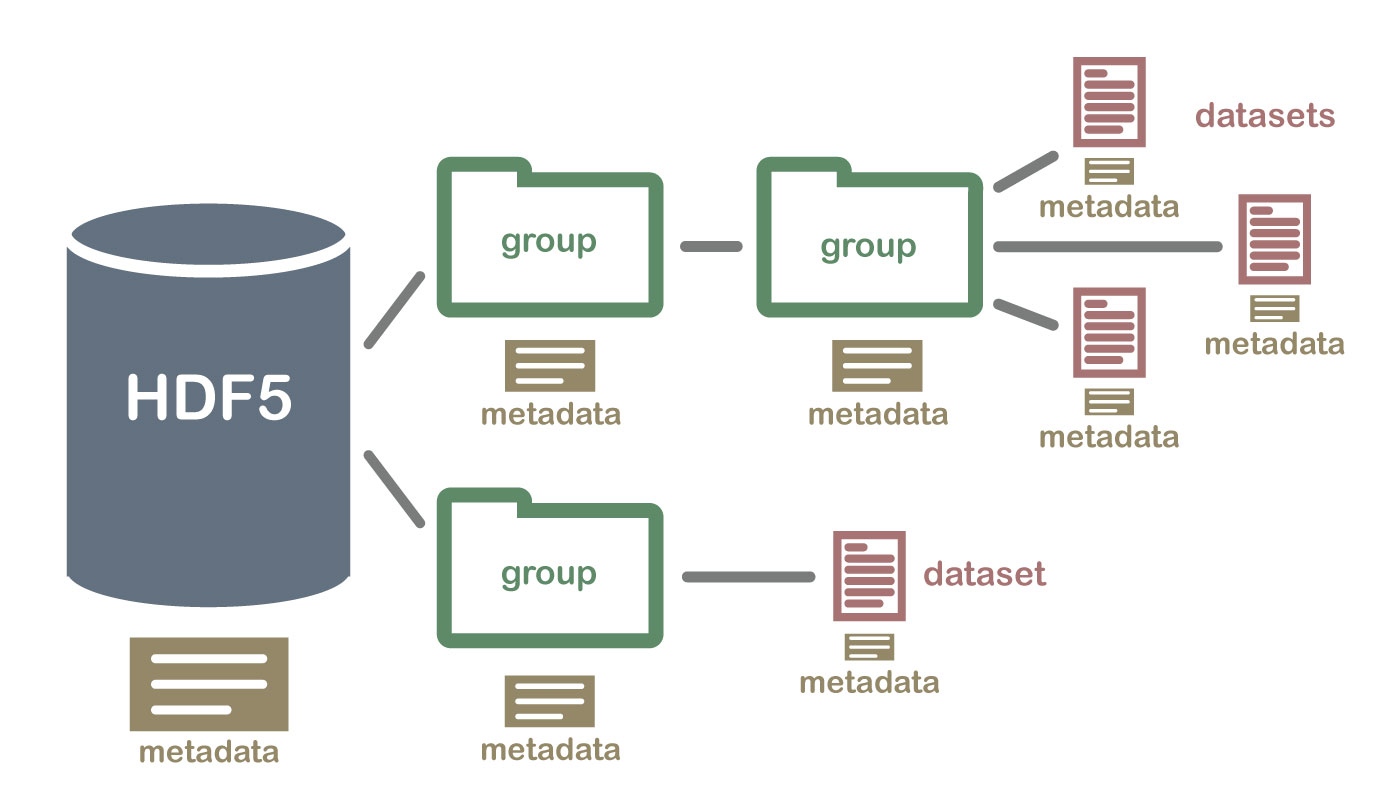
\includegraphics[width=0.5\textwidth]{hdf5_structure4}
				\caption{Diagram of the HDF5 file format, from the National Ecological Observatory Network. The metadata attached to groups and datasets are called ``attributes''.}
			\end{figure}

		\subsubsection{Components of an HDF5 File}
			\noindent The two main aspects of an HDF5 file are \textbf{groups} and \textbf{datasets}. In addition there are \textbf{attributes} that can be attached to groups and datasets.
			\begin{itemize}
				\item \textbf{Groups} define organization within the file and can optionally have associated metadata (attributes). Every HDF5 file contains a root group that can contain datasets or other groups. Working with groups is similar to working with directories and files in UNIX. For example: \texttt{/} is the root group, \texttt{/foo} is a member of the root group called \texttt{foo}, \texttt{.} signifies the specified file, group or object.\\
			Each instance of the core classes in the AOData framework (see \myurl{\ref{section:Framework}} on ``Framework'') above are written as a group in the HDF5 file.
			%\\$\quad$\\
				\item \textbf{Datasets} organize and contain ``raw'' data values. A dataset consists of the data itself and metadata (attributes) that describes the data. Most MATLAB data types have a comparable HDF5 datatype, with one exception - multi-level structures (a \aodclass{struct} where one or more fields is another \aodclass{struct} or another compound datatype like \aodclass{table} or \aodclass{containers.Map}). The details of conversion to HDF5 datatype are discussed in \ref{section:HDF5_Details}.
			%\\$\quad$\\
				\item \textbf{Attributes} can optionally be associated with HDF5 objects. They have two parts: a \textit{name} and a \textit{value}. Typically an attribute is small and contains metadata about the object it is attached to, either a group or a dataset.
			%\\$\quad$\\
				\item \textbf{References} are low-level pointers to other objects. They can be stored and retrieved as data, created as an attribute or an entire dataset of reference type.
				There are two types of references, the first is used often in AOData for links between entities.
				\begin{enumerate}
					\item \textit{Object references} point to a particular object in a file, either a dataset or a named datatype.
					\item \textit{Region references} always point to a dataset and additionally contain info about a certain selection (\textit{dataset region}) on that dataset. %For example, you could specify a region of interest and store it as an attribute on the dataset
				\end{enumerate}
			\end{itemize}
		\subsubsection{Viewing HDF5 files}
			\noindent A disadvantage of using HDF5 files is that they are binary and not human-readable (i.e. you can't pull the file up in a text editor and read it, like for a JSON file). Instead, you will need some sort of software to visualize the contents of an HDF file. The most commonly used is the HDF Group's \href{https://www.hdfgroup.org/downloads/hdfview/}{\myurl{HDFView}}. This is definitely worth installing.
			\\
			HDFView is very generic because HDF5 files can be very diverse. AOData HDF5 files are built around the AOData object model, which provides a predictable structure.
			I wrote \aodclass{AODataViewer} to be designed around the AOData framework.
			\begin{lstlisting}[style=matlab-editor, basicstyle=\mlttfamily\footnotesize]
AODataViewer('myfile.h5');
			\end{lstlisting}
			There is also a standalone compiled version that does not require a MATLAB license: \textcolor{red}{link}.

			There are a number of nice options if you're comfortable with Python, such as \href{https://github.com/ganymede42/h5pyViewer}{\myurl{h5pyViewer}} and \href{https://vitables.org}{\myurl{ViTables}}. Regardless of the language you intend to use, I recommend first looking through the files with \aodclass{AODataViewer} because it's designed to facilitate understanding the AOData framework.
			\\$\quad$\\
			\noindent \textcolor{red}{Figure here.} Understanding how AOData writes experiment data to an HDF5 file is described in \myurl{\ref{section:HDF5_Details}} on ``HDF5 File Details''. Groups are shown with folders and datasets are shown with files. Groups that are containers for multiple entities are italicized, the other groups correspond to entities. Checking out the example file will make this clearer.
	\subsection{Advanced MATLAB Concepts}
		\noindent This section has information on a few MATLAB-specific topics (other languages probably have similar things using different names) that aren't routinely covered in the introductory documentation but are critical to how AOData operates. \textit{You don't need to read and understand this prior to using AOData!} You may never need to deal with these directly; after all, the whole point of abstraction in \ref{subsection:OOP} is that complicated behind-the-scenes code is handled and kept hidden from end-users.
		At some point though as you work with AOData, you might have questions about these topics and can circle back to the information below:
	\subsubsection{Handle vs. Value Classes}\label{subsubsection:HandleValue}
		\noindent When you work with \matclass{char} and \matclass{double}, you are working with \underline{value classes}.
		\begin{lstlisting}[style=matlab-editor, basicstyle=\mlttfamily\footnotesize]
% Create a double variable
a = 3.14
% Copy it to another variable
b = a;
% Change the value of b
b = 3.14159;
% You have changed b, but not a
disp([a, b])
	\end{lstlisting}
	\noindent By contrast, most classes in AOData are \underline{handle classes}. Handle classes provide a ``handle'' to the object, which is stored only one in memory:
	\begin{lstlisting}[style=matlab-editor, basicstyle=\mlttfamily\footnotesize]
% Create a standalone Device class. It's from ThorLabs but you don't remember the Model
device1 = aod.core.Device([], 'Manufacturer', 'ThorLabs', 'Model', 'idk');
% Copy set a second variable equal to device1
device2 = device1;
% Now you remember the Model number
device2.setAttr('Model', 'P20K');
% The Model attribute is now changed for device2...
disp(device2.parameters)
% ...and for device1, because both variables were just handles to data that exists only once in memory
disp(device1.parameters)
		\end{lstlisting}
		\noindent Why is this relevant to AOData? See below:
		\begin{lstlisting}[style=matlab-editor, basicstyle=\mlttfamily\footnotesize]
% Create a channel
channel = aod.core.Channel('MyChannel');
% Create a device and add it to the channel
device = aod.core.Device('Manufacturer', 'ThorLabs', 'Model', 'idk');
channel.add(device);
% Change a attribute on the device variable
device.setAttr('Model', 'P20K');
% And it is also changed within the Channel!
disp(channel.Devices.parameters)
		\end{lstlisting}
		%See MATLAB's documentation on \href{https://www.mathworks.com/help/matlab/matlab_oop/comparing-handle-and-value-classes.html}{\myurl{Comparison of Handle and Value Classes}} for more information.

	\subsubsection{matlab.mixin.Heterogeneous}
		\label{subsubsection:Heterogeneous}
		\noindent When you create custom classes in MATLAB, you can only concatenate members of the same class. This gets annoying when you have multiple subclasses of one of your custom classes and want to make them into an array (which we do for all containers). By subclassing \matclass{matlab.mixin.Heterogenous} in each core class (other than Entity), your subclasses of, for example, \aodclass{aod.core.Device} can be concatenated into an array. A quirk of using \matclass{matlab.mixin.Heterogeneous} is that all methods in the class subclassing it must be either \texttt{Sealed} or \texttt{Abstract}. You don't have to continue this practice when subclassing the core classes and do not need to declare inheritance again from \matclass{matlab.mixin.Heterogeneous}. Also, your classes cannot inherit two classes that use \matclass{matlab.mixin.Heterogeneous} (e.g. both Device and Channel), though I can't imagine why you would need to do that anyway.
	\subsubsection{Enumerations}
		\label{subsubsection:Enum}
		\noindent Enumerations are useful when you have a list of things and you want to standardize their behavior. MATLAB's documentation (see \myurl{\ref{section:CodeDoc}}) will do a better job describing this than I will, but two things are worth mentioning here. First, entity behavior is codified in an enumeration (\aodclass{aod.common.EntityTypes}). Second, you may want to include a static \aodfcn{init} method if you want to read back your own enumerations classes from HDF to MATLAB. You don't need to deal with enumerations to use AOData, but they can be helpful (for more examples see \aodclass{sara.epochs.EpochTypes} and \aodclass{sara.SpectralTypes}).

	\subsubsection{Dynamic Properties}
		\label{subsubsection:DynProps}
		\noindent The MATLAB \aodclass{dynamicprops} class enables ad-hoc addition of properties to specific instances of a class (often called ``instance properties'' in other programming languages). The advantage of dynamic properties is that they allow the persistent interface to adapt to customized subclasses of the core classes without any prior knowledge of said subclass (other than which entity type it is).

\section{Workflow}
	\label{section:Workflow}
	\noindent To use AOData for an experiment, you will follow the workflow below.
	\begin{enumerate}
		\item Define how your experiment will map to the AOData object model in MATLAB using the Core Interface (see \myurl{\ref{section:CoreInterface}}). Creating the subclasses will require an initial investment, after which users will only need to work in the core interface when changes are made to an experiment.
		\item Experiment specification file (example).
		\item Write your experiment to the HDF5 file with \aodfcn{aod.h5.writeExperimentToFile}.
		\item Once you have the HDF5 file, you can continue your analysis in any language you would like. If you choose to use MATLAB for analysis, you will access your HDF5 file through the Persistent Interface (see \myurl{\ref{section:PersistentInterface}}). You can still make changes to the HDF5 file at this point and the techniques for doing so are defined below.
	\end{enumerate}
	\noindent You will need to define subclasses of the core classes to define how exactly you want your experiment to be set up. This will require an initial investment of time to set the classes up. Once established, it is unlikely you will need to modify these unless you change up how you're performing your experiments (which can often mean different data types, metadata and/or parameters).

\section{Core Interface}
	\label{section:CoreInterface}
	\noindent This information is compiled here to serve as a single resource for core classes. It may not be the best gateway for learning about the core classes for the first time. If the documentation below seems like too much information, try to read through \myurl{\ref{subsection:EntityDoc}} on \aodclass{aod.core.Entity} and then read \myurl{\ref{subsection:ClassDesign}} on ``Class Design Principles'', before returning.  However, each class and function is thoroughly documented in the source code. For more detail on any aspect below, try using the \matfcn{help} command in MATLAB:
	\begin{lstlisting}[style=matlab-editor, basicstyle=\mlttfamily\footnotesize]
% Get documentation for a class or function
help aod.core.Experiment
% Get documentation for a function within a class
help aod.core.Experiment\add
	\end{lstlisting}
	\noindent The documentation for each class includes (if relevant), the following information:\smallskip\\
	\textbf{className \myparent{parentClassName(s)}}\smallskip\\
	The constructor will be shown. There may be two version, one with the minimal number of required inputs and a second showing the optional inputs.
	\begin{lstlisting}[style=matlab-editor, basicstyle=\mlttfamily\footnotesize]
obj = MyClass(inputs)
	\end{lstlisting}
	\docheader{Properties:} - Class properties that are written as datasets, with two exceptions: \aodclass{aod.core.Entity}'s properties are written as parameters and anything designated as a container is a group that contains other entities. %Anything designated as a link, will be written as a link
	\begin{itemize}
		\item \aodprop{MyProp}
	\end{itemize}
	\docheader{Parameters:} Optional inputs sent to \aodclass{aod.common.KeyValueMap} and written as attributes
	\begin{itemize}
		\item \aodparam{MyParam}
	\end{itemize}
	\docheader{Methods:}
	\begin{itemize}
		\item \aodfcn{outputs = MyFcn(obj, inputs)}
	\end{itemize}
	\docheader{Examples:} Subclasses within AOData that demonstrate implementation
	\begin{itemize}
		\item \aodclass{SubclassName}
	\end{itemize}
	\noindent Methods may be listed with some combination of Abstract, Sealed, Static, Protected or Private. Properties may be listed as Abstract, Dependent, Protected or Private. If access isn't specified, assume it is Public. If these terms aren't familiar, check out the resource recommendations in \myurl{\ref{subsection:OOP}} on ``Object Oriented Programming''.

	\subsection{ao.core.Entity \textcolor{gray}{(handle)}}
		\label{subsection:EntityDoc}
		\noindent  Abstract parent class to all core classes that are persisted into the HDF5 file. Because all core classes inherit \aodclass{aod.core.Entity}, they all operate in a similar way and if you learn the basics of this parent class, you'll already need to know most of how the subclasses work.

		Before getting into the code documentation, it is worth explaining it in the context of AOData's goals. The main question in designing \aodclass{aod.core.Entity} was: What should all components have in common? and How can they be implemented in a flexible/generic way to avoid unnecessarily restricting subclasses? In an ideal world, \aodclass{aod.core.Entity} will be set in stone as any change here will change the rest of the framework. So it needs to provide enough options (optional options, not required options - you should be able to use what you want and ignore the rest) to be robust and flexible. To ensure end-users aren't depending on critical functionality, the things that \aodclass{aod.core.Entity} absolutely \textit{must} do to make the code work should be hidden from the average user.
		\begin{lstlisting}[style=matlab-editor, basicstyle=\mlttfamily\footnotesize]
% Note that aod.core.Entity is abstract and never directly instantiated.
% This is the constructor that subclasses will call in their constructors
obj = aod.core.Entity(name)
		\end{lstlisting}
		\docheader{Properties:}
		\begin{itemize}
			\item \aodprop{Name} - user-defined name for the entity
			\item \aodprop{description} - a space for describing the Entity is (in case the class, properties and parameters are not sufficient)
			\item \aodprop{parameters} - \aodclass{aod.common.KeyValueMap} containing entity metadata
			\item \aodprop{files} - \aodclass{aod.common.KeyValueMap} containing file names associated with the entity
			\item \aodprop{notes} - a space for miscellaneous comments
		\end{itemize}
		\docheader{Private Properties:} These are handled behind the scenes and average users shouldn't need to worry about them
		\begin{itemize}
			\item \aodprop{Parent} optional, another entity that the current entity falls under in the  hierarchy (e.g. the Parent for an Epoch is the Experiment). This is set when you add the entity to another entity using \aodfcn{add()}.
			\item \aodprop{UUID} - a randomly-generated unique identifier from \aodfcn{aod.util.generateUUID()}. Behind the scenes, these are used to search through entities and their HDF5 counterparts, providing a solution for indexing which is one of HDF5's larger shortcomings. See \myurl{\ref{subsubsection:EntityManager}} on \aodclass{aod.h5.EntityManager} for the solution.
		\end{itemize}
		\docheader{Dependent Properties:}
		\begin{itemize}
			\item \aodprop{label} - automatically generated label based on data and metadata. Set to the output of \aodfcn{specifyLabel()}
		\end{itemize}
		\docheader{Public methods:}
		\begin{itemize}
			\item \aodfcn{setDescription(obj, txt)}
			\item \aodfcn{setNote(obj, txt)}
			\item \aodfcn{removeNote(obj, ID), \aodfcn{removeNote(obj, 'all')}}\\
			%
			\item \aodfcn{add(obj, entity)} - Add an entity\\
			%
			\item \aodfcn{tf = hasAttr(obj, 'paramName')}
			\item \aodfcn{addParam(obj, 'paramName', paramValue)} - add parameters as key/value pair(s) or a struct
			\item \aodfcn{removeAttr(obj, paramName)}
			\item \aodfcn{paramValue = getAttr(obj, 'paramName', mustReturnParam)}\\
			%
			\item \aodfcn{tf = hasFile(obj, fileKey)}
			\item \aodfcn{setFile(obj, fileKey, filePath)}
			\item \aodfcn{fileValue = getFile(obj, fileKey)}
			\item \aodfcn{fileValue = getExpFile(obj, fileKey)} - appends the current \aodprop{homeDirectory} to the returned file path
			\item \aodfcn{removeFile(obj, fileKey)}\\
			%
			\item \aodfcn{fPath = getHomeDirectory(obj)} - once an entity has been added to the Experiment or to another entity that is added, this function will return the \aodprop{homeDirectory} of \aodclass{aod.core.Experiment}
			\item \aodfcn{h = getParent(obj, entityType)} - recursively searches \aodprop{Parent} to find an entity of the specified type. % find an entity that that is a className or subclass of className
			\item \aodfcn{assignUUID(obj, UUID)} - assign a specific UUID to an entity. UUIDs are generated automatically for all entities and must be unique within in an experiment. However, some entities may not be unique across experiments. Use this method if you would like to have, for example, a Source or Device that is identifiable by the same UUID in each experiment.
		\end{itemize}
		\docheader{Protected methods:}
		\begin{itemize}
			\item \aodfcn{value = specifyLabel(obj)} - defines \aodprop{label}. Default value is the class name without packages but subclasses should tailor it, if needed.
			\item \aodfcn{setParent(obj, entity)}
			\item \aodfcn{sync(obj)} - For updating entity after added to the main experiment hierarchy. Use this is the entity needs information from other entities (e.g. \aodprop{Parent})
		\end{itemize}

	\subsection{aod.core.Experiment  \myparent{aod.core.Entity}}
		\noindent The parent class for all other entities, containing everything associated with a specific experiment. Experiment is written first to the HDF5 file and the other entities are written in the order shown below.

		\begin{lstlisting}[style=matlab-editor, basicstyle=\mlttfamily\footnotesize]
obj = aod.core.Experiment('name', experimentDate, 'homeDirectory')
obj = aod.core.Experiment('name', experimentDate, 'homeDirectory',...
	'Administrator', "YourName", 'System', "Primate1P")
		\end{lstlisting}
		\docheader{Properties:}
		\begin{itemize}
			\item \aodprop{homeDirectory} - file path to experiment folder
			\item \aodprop{experimentDate} - date that the experiment occurred (yyyyMMdd)
			\item \aodprop{Analyses} - container for all Analyses within the Experiment
			\item \aodprop{Calibrations} - container for all Calibrations within the Experiment
			\item \aodprop{Epochs} - container for all Epochs within the Experiment
			\item \aodprop{Sources} - container for all Sources within the Experiment
			\item \aodprop{Annotations} - container for all Annotations within the Experiment
			\item \aodprop{Systems} - container for all Systems within the Experiment
		\end{itemize}
		\docheader{Dependent Properties:}
		\begin{itemize}
			\item \aodprop{epochIDs} - the IDs of all epochs in Experiment
			\item \aodprop{numEpochs} - the number of epochs in the Experiment
		\end{itemize}
		\docheader{Parameters:}
		\begin{itemize}
			\item \aodparam{Administrator} - who performed the experiment
			\item \aodparam{System} - the name of they system used
		\end{itemize}
		\docheader{Methods:} This may seem like a lot, but many of the methods are conceptually identical (e.g. if you know how to use \aodfcn{add}, then you know how to use all the add methods)
		\begin{itemize}
			\item \aodfcn{setHomeDirectory(obj, filePath)} - change file path to experiment data folder
			\item \aodfcn{add(obj, entity)} - add Analysis, Annotation, Calibration, Epoch, Annotation, Source or System
			\item \aodfcn{remove(obj, entity, ID)} - remove an Analysis, Annotation, Calibration, Epoch, Source or System. ID should be the index of the entity/entities (or epochID for Epochs) to remove or "all" to clear all \\
			%
			\item \aodfcn{epoch = id2epoch(obj)} - input ID and returns Epoch, if exists
			\item \aodfcn{idx = id2index(obj, ID)} - input ID and return the index of the Epoch in Epochs \\
		\end{itemize}
	\subsection{aod.core.Source \myparent{aod.core.Entity, matlab.mixin.Heterogeneous}}
		\label{subsection:aod.core.Source}
		\noindent The source of the data acquired during the experiment.
		\begin{lstlisting}[style=matlab-editor, basicstyle=\mlttfamily\footnotesize]
obj = aod.core.Source(parent, 'name')
		\end{lstlisting}
		\docheader{Sealed Methods:}
		\begin{itemize}
			\item \aodfcn{add(obj, source)} - add source
			\item \aodfcn{remove(obj, sourceID)} - remove a child source
			\item \aodfcn{clearChildSources(obj)} - clear all child sources
			\item \aodfcn{sources = getParents(obj)}
			\item \aodfcn{ID = getParentID(obj)}
		\end{itemize}

		\noindent Sources are nestable. For an example hierarchy, see the following Source subclasses where you might have 2 locations in 1 eye of 1 subject.
		When specifying the source for \aodclass{aod.core.Epoch}, use the most specific Source in the hierarchy.
		\subsubsection{aod.core.sources.Subject \textcolor{gray}{(aod.core.Source)}}
			\noindent Top-level source (person, monkey, mouse, model eye).
			\begin{lstlisting}[style=matlab-editor, basicstyle=\mlttfamily\footnotesize]
obj = aod.core.Subject(name)
obj = aod.core.Subject(name, 'Species', value, 'Sex', value, 'Demographics', value)
			\end{lstlisting}
			\docheader{Parameters:}
			\begin{itemize}
				\item \aodparam{Species}
				\item \aodparam{Sex} - male, female or unknown
				\item \aodparam{Age}
				\item \aodparam{Demographics} - fluorophore, transgenic line, disease
			\end{itemize}
		\subsubsection{aod.core.sources.Eye \textcolor{gray}{(aod.core.Source)}}
			\noindent An Eye within the Subject. \aodprop{Name} is restricted to being either OS or OD.
			\begin{lstlisting}[style=matlab-editor, basicstyle=\mlttfamily\footnotesize]
obj = aod.core.sources.Eye(name)
			\end{lstlisting}
			\docheader{Properties:}
			\begin{itemize}
				\item \aodprop{name} - inherited from Entity, but with added restriction of being either 'OS' or 'OD'
			\end{itemize}

		\subsubsection{aod.core.sources.Location  	\textcolor{gray}{(aod.core.Source)}}
			\noindent A location within an Eye.
			\begin{lstlisting}[style=matlab-editor, basicstyle=\mlttfamily\footnotesize]
obj = aod.core.sources.Location(name)
			\end{lstlisting}

	\subsection{aod.core.Calibration \myparent{aod.core.Entity, matlab.mixin.Heterogeneous}}
		\label{subsection:CalibrationDoc}
		\noindent Represents measurements of the system (e.g. spectra/power of light sources, optimized positions of PMT). %I added a few built-in classes for standard calibrations (e.g. \aodclass{aod.builtin.calibrations.PowerMeasurement}) that could be good references on how to implement this class.

		\begin{lstlisting}[style=matlab-editor, basicstyle=\mlttfamily\footnotesize]
obj = aod.core.Calibration(name, calibrationDate)
		\end{lstlisting}
		\docheader{Properties:}
		\begin{itemize}
			\item \aodprop{calibrationDate} - date calibration was performed
		\end{itemize}
		\docheader{Methods:}
		\begin{itemize}
			\item \aodfcn{setDate(obj, calDate)} - calDate should be \aodclass{datetime} or a \aodclass{char} with the format yyyyMMdd
		\end{itemize}
		\docheader{Examples:}
		\begin{itemize}
			\item \aodclass{aod.builtin.calibrations.PowerMeasurement}
			\item \aodclass{aod.builtin.calibrations.RoomMeasurement}
			\item \aodclass{aod.builtin.calibrations.ChannelOptimization}
		\end{itemize}
	\subsection{aod.core.System \myparent{aod.core.Entity, matlab.mixin.Heterogeneous}}
		\label{subsection:SystemDoc}
		\noindent Represents the system configuration you used to acquire the data. While there is only one system, you may use it in different ways within or between experiments, depending on the type of imaging your're doing. The reasoning behind this organization is that you may used one system in two different ways during an experiment (e.g. calcium imaging requires a different set of channels than rhodamine imaging)

		\begin{lstlisting}[style=matlab-editor, basicstyle=\mlttfamily\footnotesize]
obj = aod.core.System(name)
		\end{lstlisting}
		\noindent Because it is hard to automate system names, \texttt{name} is a required input

		\docheader{Properties:}
		\begin{itemize}
			\item \aodprop{Channels} - container for all \aodclass{aod.core.Channel}s within the System
		\end{itemize}
		\docheader{Sealed Methods:}
		\begin{itemize}
			\item \aodfcn{add(obj, channel)} - Add a Channel to the system
			\item \aodfcn{remove(obj, ID)} - ID is the index of the channel to remove. The standard remove syntax is also accepted: \aodfcn{remove(obj, entityType, ID)}, but entityType must be Channel
			\item \aodfcn{getChannelDevices(obj)}
		\end{itemize}

	\subsection{aod.core.Channel \myparent{aod.core.Entity, matlab.mixin.Heterogeneous}}
		\label{subsection:ChannelDoc}
		\noindent A single light path within the System. For example, the calcium imaging channel contains a Mustang laser, a bandpass filter, a PMT and a pinhole. The specifics of these devices may change between experiments (for example, you may test different pinhole sizes for fluorescence imaging) or even within experiments (trying out different dichroic filters).

		\begin{lstlisting}[style=matlab-editor, basicstyle=\mlttfamily\footnotesize]
obj = aod.core.Channel(name)
		\end{lstlisting}

		\docheader{Properties:}
		\begin{itemize}
			\item \aodprop{Devices} - container for all \aodclass{aod.core.Device}s within the Channel
		\end{itemize}
		\docheader{Sealed Methods:}
		\begin{itemize}
			\item \aodfcn{add(obj, device)} - Add a Device to the channel
			\item \aodfcn{removeDevice(obj, ID)}
			\item \aodfcn{clearDevices(obj)}
		\end{itemize}

	\subsection{aod.core.Device  \myparent{aod.core.Entity, matlab.mixin.Heterogeneous}}
		\noindent Any sort of Device within a Channel worth logging. You don't necessarily need to add every single mirror in the light path, just the components that are critical and may have parameters that change between experiments. See \myref{subsection:ClassDesign} on ``Class Design'' for a thorough explanation of how this class was designed that introduces the principles behind all other core classes.

		\begin{lstlisting}[style=matlab-editor, basicstyle=\mlttfamily\footnotesize]
obj = aod.core.Device(name)
obj = aod.core.Device(name, 'Model', value, 'Manufacturer', value);
		\end{lstlisting}
		\docheader{Parameters:}
		\begin{itemize}
			\item \aodparam{Manufacturer}
			\item \aodparam{Model}
		\end{itemize}
		\docheader{Examples:}
		\begin{itemize}
			\item \aodclass{aod.builtin.devices.BandpassFilter}
			\item \aodclass{aod.builtin.devices.DichroicFilter}
			\item \aodclass{aod.builtin.devices.LightSource}
			\item \aodclass{aod.builtin.devices.Pinhole}
			\item \aodclass{aod.builtin.devices.PMT}
		\end{itemize}

	\subsection{aod.core.Annotation \myparent{aod.core.Entity, matlab.mixin.Heterogeneous}}
		\noindent Spatial regions within your acquired data. These could be ROIs in a physiology experiment, coordinates of labeled cells in anatomical imaging or a subregion of the field of view that omits the zeroed pixels after registration.

		\begin{lstlisting}[style=matlab-editor, basicstyle=\mlttfamily\footnotesize]
obj = aod.core.Annotation()
obj = aod.core.Annotation(data)
		\end{lstlisting}
		\docheader{Properties:}
		\begin{itemize}
			\item \aodprop{Data}
			\item \aodprop{Source}
		\end{itemize}
		\docheader{Protected Properties:}
		\begin{itemize}
			\item \aodprop{Reader} - \aodclass{aod.common.FileReader}
		\end{itemize}
		\docheader{Sealed Protected Methods:}
		\begin{itemize}
			\item \aodfcn{setData(obj, data)}
			\item \aodfcn{setSource(obj, source)}
		\end{itemize}
		\docheader{Examples:}
		\begin{itemize}
			\item \aodclass{aod.builtin.annotations.Rois}
		\end{itemize}

	\subsection{aod.core.Epoch \myparent{aod.core.Entity, matlab.mixin.Heterogeneous}}
		\noindent A single period of data acquisition within the Experiment. Epochs differ from the other entities in one key way: because they already have an intuitive numeric identifier (\aodprop{ID}, the video number in the experiment), this is used rather than their index in the \aodprop{Epochs} container for methods like \aodfcn{remove()}

		\begin{lstlisting}[style=matlab-editor, basicstyle=\mlttfamily\footnotesize]
obj = aod.core.Epoch(ID)
		\end{lstlisting}
		\docheader{Properties:}
		\begin{itemize}
			\item \aodprop{ID} - (required) number of epoch within the experiment. ID must be an integer, though not necessarily consecutive, to facilitate indexing and sorting of Epochs. If you have some other non-integer specification for individual trials, your subclasses can use the \aodfcn{setName()} function to define that convention and assign it to \aodprop{Name}.
			\item \aodprop{startTime} - time the epoch started (\aodclass{datetime})\\
			%
			\item \aodprop{Timing} - timestamps for data acquisition during the epoch
			\item \aodprop{Registrations} - container for \aodclass{aod.core.Registration}
			\item \aodprop{Responses} - container for \aodclass{aod.core.Response}
			\item \aodprop{Stimuli} - container for \aodclass{aod.core.Stimulus}
			\item \aodprop{Datasets} - container for \aodclass{aod.core.Dataset}
			\item \aodprop{Source} - link to \aodclass{aod.core.Source} for the Epoch
			\item \aodprop{System} - link to \aodclass{aod.core.System} for the Epoch
		\end{itemize}
		\docheader{Sealed Methods:}
		\begin{itemize}
			\item \aodfcn{setSource(obj, system)}
			\item \aodfcn{setSystem(obj, system)}\\
			%
			\item \aodfcn{add(obj, entity)} - Add a Dataset, Registration, Response or Stimulus to the Epoch
			\item \aodfcn{remove(obj, entityType, ID)} - Remove...
			\item \aodfcn{get(obj, entityType, varargin)}
			%
		\end{itemize}

	\subsection{aod.core.Registration \myparent{aod.core.Entity, matlab.mixin.Heterogeneous}}
		\noindent Any registration applied to the raw data acquired during an Epoch. For example, if you use Qiang's registration software, you can use \aodclass{aod.builtin.registrations.StripRegistration} to store the metadata and specify whether you used frame or strip.

		\begin{lstlisting}[style=matlab-editor, basicstyle=\mlttfamily\footnotesize]
obj = aod.core.Registration(name, registrationDate)
		\end{lstlisting}
		\docheader{Properties:}
		\begin{itemize}
			\item \aodprop{registrationDate} - date registration was performed
		\end{itemize}
		\docheader{Methods:}
		\begin{itemize}
			\item \aodfcn{setDate(obj, regDate)}
		\end{itemize}
		\docheader{Examples:}
		\begin{itemize}
			\item \aodclass{aod.builtin.registrations.RigidRegistration}
			\item \aodclass{aod.builtin.registrations.StripRegistration}
		\end{itemize}
	\subsection{aod.core.Stimulus \myparent{aod.core.Entity, matlab.mixin.Heterogeneous}}
		\noindent Stimuli presented during the Epoch. Optionally, the contents of \aodclass{aod.core.Stimulus} can be generated automatically by passing a \aodclass{aod.common.Protocol} used to create the stimulus presented during the trial.
		\begin{lstlisting}
obj = aod.core.Stimulus(name)
obj = aod.core.Stimulus(name, protocol)
		\end{lstlisting}
		\docheader{Properties:}
		\begin{itemize}
			\item \aodprop{Calibration} - \aodclass{aod.core.Calibration} used to design the stimulus, if applicable
			\item \aodprop{protocolClass}
			\item \aodprop{protocolName}
		\end{itemize}
		\docheader{Methods:}
		\begin{itemize}
			\item \aodfcn{setCalibration(obj, calibration)} - Set Calibration used, if wasn't already extracted from Protocol
			\item \aodfcn{setProtocol(obj, protocol)} - Set protocol, if wasn't already passed as an input to the constructor
			\item \aodfcn{protocol = getProtocol(obj)}
		\end{itemize}
		\docheader{Examples:}
		\begin{itemize}
			\item \aodclass{aod.builtin.stimuli.ImagingLight} - Example of stimulus defined without a Protocol
		\end{itemize}

	\subsection{aod.core.Dataset \myparent{aod.core.Entity, matlab.mixin.Heterogeneous}}
		\noindent Space for storing datasets acquired during the Epoch. Could be the acquired videos if you would like to store them in the HDF5 file, or some other ``meta-dataset'' related to the Epoch, like information about the wavefront sensing. If there is just one thing being saved, consider setting it to \aodprop{Data} for consistency. If there are multiple things being saved, your subclasses can add additional properties, or ignore \aodprop{Data} all together if it doesn't make sense for your purpose (empty properties will not be saved to the HDF5 file and are not required for reading the entities back in).
		\begin{lstlisting}
obj = aod.core.Dataset(name)
obj = aod.core.Dataset(name, data)
		\end{lstlisting}
		\docheader{Properties:}
		\begin{itemize}
			\item \aodprop{Data}
		\end{itemize}
		\docheader{Sealed Protected Methods:}
		\begin{itemize}
			\item \aodfcn{setData(obj, data)}
		\end{itemize}

	\subsection{aod.core.Response \myparent{aod.core.Entity, matlab.mixin.Heterogeneous}}
		\noindent A time-varying signal extracted from the data acquired during an Epoch. You can set \aodprop{Timing} if it differs from the timing set at the \aodclass{Epoch} level, otherwise it will be written as a link to Epoch's \aodprop{Timing}
		\begin{lstlisting}[style=matlab-editor, basicstyle=\mlttfamily\footnotesize]
obj = aod.core.Response(name)
		\end{lstlisting}
		\docheader{Properties:}
		\begin{itemize}
			\item \aodprop{Data}
			\item \aodprop{Timing} - inherited from \aodclass{aod.core.Epoch}'s \aodprop{Timing} if unset
		\end{itemize}
		\docheader{Sealed Methods:}
		\begin{itemize}
			\item \aodfcn{setData(obj, data)}
			\item \aodfcn{addTiming(obj, timing)}
		\end{itemize}

		\docheader{Examples:}
		\begin{itemize}
			\item \aodclass{aod.builtin.responses.RegionResponse}
			\item \aodclass{sara.responses.Dff}
			\item \aodclass{sara.responses.Fluorescence}
		\end{itemize}
		\noindent Keep in mind that you can set the \aodprop{Parent} prior to adding the response to an Epoch. This is often needed for initializing a Response, as information from the parent Epoch might be required. All of the examples above take this approach and can be used as reference.

		\subsubsection{aod.core.responses.RegionResponse \myparent{aod.core.Response}}
			\noindent A Response associated with an instance of \aodclass{aod.core.Annotation}.
			\begin{lstlisting}[style=matlab-editor, basicstyle=\mlttfamily\footnotesize]
obj = aod.core.responses.RegionResponse(parent, varargin)
			\end{lstlisting}

	\subsection{aod.core.Analysis \myparent{aod.core.Entity, matlab.mixin.Heterogeneous}}
		\noindent Represents any analysis performed on entities within the Experiment. This class standardizes recording of the entities analyzed, otherwise it's a blank slate to fill in with the implementation. Placing your code within an Analysis class allows you to save both the results of the analysis and how the results were generated.
		\begin{lstlisting}[style=matlab-editor, basicstyle=\mlttfamily\footnotesize]
obj = aod.core.Analysis('name')
obj = aod.core.Analysis('name', analysisDate)
		\end{lstlisting}
		\docheader{Properties:}
		\begin{itemize}
			\item \aodprop{analysisDate} - date analysis was performed
		\end{itemize}
		\docheader{Methods:}
		\begin{itemize}
			\item \aodfcn{setDate(obj, analysisDate)}
		\end{itemize}
	\subsection{Quick Reference}
		\noindent A quick overview of classes and constructors:
		\begin{lstlisting}[style=matlab-editor, basicstyle=\mlttfamily\footnotesize]
experment = aod.core.Experiment(name, homeFolder, experimentDate);
experment = aod.core.Experiment(name, homeFolder, experimentDate, 'Administrator', "adminName", 'System', "systemName");

obj = aod.core.Source(name)

system = aod.core.System('systemName');

channel = aod.core.Channel('channelName');

device = aod.core.Device('name');
device = aod.core.Device('name', 'Manufacturer', "manufacturerName", 'Model', "modelName");

calibration = aod.core.Calibration('name', calibrationDate);
calibration = aod.core.Calibration('name', calibrationDate, "Administrator", "adminName");

epoch = aod.core.Epoch(ID);
epoch = aod.core.Epoch(ID, 'Source', value, 'System', value);

registration = aod.core.Registration('name', regDate)
registration = aod.core.Registration('name', regDate, "Administrator", "adminName")

stimulus = aod.core.Stimulus(name);
stimulus = aod.core.Stimulus(name, protocol);

dataset = aod.core.Dataset(name);
dataset = aod.core.Dataset(name, data);

response = aod.core.Response(name);
		\end{lstlisting}

\section{Support Classes}
	\subsection{aod.common.EntityTypes \myparent{enumeration}}
		\noindent Lays out the business logic of the different entity types. Unlikely that you will need to make any changes here but it's worth checking out if you're interested in how the entities are organized.

	\subsection{aod.util.Factory \textcolor{gray}{(handle)}}
		\noindent Factory classes simplify the creation of standardized entities. For example, if you have some standard Devices you frequently use, you could subclass Device and create a class for each or you could create a pipeline with Factory to keep OOP from getting out of control. See \aodclass{sara.factories.ChannelFactory} for an example.

		Factory is an abstract class with two abstract methods, a public \aodfcn{get()} method and a static \aodfcn{create()} method. The \aodfcn{get()} method is where your implementation goes: define the parameters you want to provide and how you will use them to return a specific entity.
		\begin{lstlisting}[style=matlab-editor, basicstyle=\mlttfamily\footnotesize]
% Instantiate the object
obj = MyFactory();
% Get the entity based on some number of inputs
entity = get(obj, varargin)
		\end{lstlisting}
		Sometimes you might want to have some properties associated with your Factory class, which means you need to instantiate the object before calling \aodfcn{get()}. If you're lazy like me and don't want to always be instantiating first, especially for factories that have no associated properties, there's the static \aodfcn{create()} method, which wraps the two lines above.
		\begin{lstlisting}[style=matlab-editor, basicstyle=\mlttfamily\footnotesize]
% Get the entity using create
entity = MyFactory.create(varargin);
		\end{lstlisting}
		Here's a blueprint for a Factory class showing \aodfcn{get()} and \aodfcn{create()}.
		\begin{lstlisting}[style=matlab-editor, basicstyle=\mlttfamily\footnotesize]
classdef MyFactory < aod.util.Factory
	methods
		function obj = get(varargin)
			% Implementation: use parameters to return a specific entity
		end
	end

	methods (Static)
		function entity = create(varargin)
			obj = MyFactory();
			entity = obj.get(varargin);
		end
	end
end
		\end{lstlisting}

	\subsection{aod.common.KeyValueMap \myparent{containers.Map}}
		\noindent  This is a wrapper for MATLAB's builtin \aodclass{containers.Map} class, so you if know how to use that then you know how to use \aodclass{aod.common.KeyValueMap}. The only differences are better command line display (each key and the associated values are displayed) and a standardized approach for writing to HDF5 files.

		This class is central to AOData because it provides a means of defining properties for entities in a flexible way that avoids hard-coding and class incompatibility as you change the underlying code.
		Each core class has a \aodclass{aod.common.KeyValueMap} class. The contents of an \aodclass{aod.common.KeyValueMap} property will be written as \textbf{attributes} of its parent entity in the HDF5 file. The contents of an attribute should be reasonably small (some text, a number, maybe a short row of numbers. If needed, more info can be found in \myurl{\ref{subsection:HDFIO}} on "Reading and Writing Entities to HDF5 files").  \textbf{In general, entity parameters are metadata and entity properties are data}. There are undoubtedly exceptions, but it's a good rule of thumb.

		\textit{More info here.} See \aodclass{aod.core.Devices} for an example on specification of default class parameters.

		There is one other use for \aodclass{aod.common.KeyValueMap} and that is providing a \aodclass{containers.Map}-like data type to store files associated with an entity (e.g. \aodprop{files} for \aodclass{aod.core.Epoch}). Any property named \aodprop{files} will be written as a group with the contents as attributes. This is a bit odd but it was the best option available as I didn't want to clutter up the entity attributes or datasets with a bunch of file names.

	\subsection{aod.util.template.ExpectedParameter \myparent{handle}}
		\label{subsection:ExpectedParameter}

		Expected parameters are provided to the \aodclass{aod.util.ParameterManager} present in \aodprop{expectedAttributes} property of every subclass of \aodclass{aod.core.Entity}.

		AOData users do not need to directly create expected parameters and can instead provide the inputs to the \aodfcn{add} method of \aodclass{aod.util.ParameterManager}.

	\subsection{aod.util.ParameterManager \myparent{handle}}
		\label{subsection:ParameterManager}
		\noindent The ParameterManager class provides users with an opportunity to specify which parameters the entity should have.
		Each AOData class inheriting from \aodclass{aod.core.Entity} has a dependent property called \aodprop{expectedAttributes}, which is set by the output of the function \aodfcn{specifyAttributes}.

		No parameters are set in \aodclass{aod.core.Entity}; however, several core classes define them. For example, \aodclass{aod.core.Device} has two expected parameters (Manufacturer and Model), which are defined as follows:

    %* TODO: Update!
		\begin{lstlisting}[style=matlab-editor, basicstyle=\mlttfamily\footnotesize]
function value = specifyAttributes()
	% Subclasses should always call the inherited method first, putting their
	% superclass after the @.
	value = specifyAttributes@aod.core.Entity()
	% Add two new parameters
	value.add('Manufacturer', [], @ischar, 'Manufacturer of the Device');
	value.add('Model', [], @ischar, 'Model of the Device');
end
		\end{lstlisting}
		When you create a device, you will see both listed in the \aodprop{expectedAttributes} property
		\begin{lstlisting}[style=matlab-editor, basicstyle=\mlttfamily\footnotesize]
device = aod.core.Device("TestDevice");
disp(device.expectedAttributes)

ParameterManager with 2 parameters:
	Model: "Default = [], Validation = @ischar, Description = []"
	Manufacturer: "Default = [], Validation = @ischar, Description = []"
		\end{lstlisting}


	\subsection{aod.common.Protocol \myparent{handle}}
		\label{subsection:ProtocolDoc}
		\noindent Protocols define how stimuli are constructed from a basic set of parameters and how they are transformed into the format the stimulator requires. See \myurl{\ref{subsection:CreatingAProtocol}} on ``Creating A Protocol'' for a detailed explanation.
		\begin{lstlisting}[style=matlab-editor, basicstyle=\mlttfamily\footnotesize]
obj = aod.common.Protocol(calibration, varargin)
		\end{lstlisting}

		\docheader{Abstract Methods:}
		\begin{itemize}
			\item \aodprop{sampleRate} - the rate data is acquired (Hz)
			\item \aodprop{stimRate} - the rate stimuli are presented (Hz)
		\end{itemize}
		\docheader{Properties:}
		\begin{itemize}
			\item \aodprop{Calibration}
			\item \aodprop{dateCreated}
			\item \aodprop{lastModified}
		\end{itemize}
		\docheader{Abstract Methods:}
		\begin{itemize}
			\item \aodfcn{stim = generate(obj)}
			\item \aodfcn{writeStim(obj, fName)}
			\item \aodfcn{value = samples2sec(obj)}
		\end{itemize}
		\docheader{Methods:}
		\begin{itemize}
			\item \aodfcn{value = sec2pts(obj)}
			\item \aodfcn{value = pts2sec(obj)}
			\item \aodfcn{value = sec2samples(obj)}
			\item \aodfcn{value = samples2sec(obj)}
		\end{itemize}

		\noindent How is \aodclass{aod.common.Protocol} different from \aodclass{aod.core.Stimulus}? A Protocol defines how the stimulus was created and provides a record of the parameters used. A Stimulus is what actually happened during the experiment (e.g. for the LEDs we have two outputs: a JSON file with the LED voltages at each stimulation interval which is 2 ms and a CSV file with the voltages at each frame along with the timing of each frame).

	\subsection{aod.common.FileReader \myparent{handle}}
		\label{subsection:FileReaderDoc}
		\noindent FileReader classes provide a designated, contained location for reading files. Create one per metadata file you want to read in, then you can easily add/remove/alter how the files are read without disrupting any other code. The files created during an experiment change with the type of trial you run and with subclasses of \aodclass{aod.core.Epoch}, you can define exactly which are needed.

		Without knowing the contents of your files and the information you want to extract, how can \aodclass{aod.common.FileReader} help you read files in a robust way, beyond just providing a contained location for reading each file?

	\subsection{aod.util.FileManager \myparent{handle}}
		\noindent The \aodclass{aod.util.FileManager} class houses pipelines for automatically identifying specific experiment files. Not every file need to be assigned through \aodclass{aod.util.FileManager}, but if you have a large number of files generated per Epoch, for example, it can be useful to segregate file name buil\\
		\docheader{Examples:}
		\begin{itemize}
			\item \aodclass{sara.util.EpochFileManager}
		\end{itemize}

	\subsection{aod.util.InputParser \myparent{inputParser}}
		\label{subsection:InputParserDoc}
		\noindent A wrapper for the MATLAB's builtin \matclass{inputParser} class that simplifies setting three defaults that would otherwise need to be retyped with every class that has optional parameter inputs. If you know how to use \matclass{inputParser}, then you know how to use \aodclass{aod.util.InputParser} (see \myurl{\ref{section:CodeDoc}} for relevant documentation - mostly you need \matfcn{addParameter}).\\
		Why are these defaults important? You don't need to know this to use AOData, but in case you're wondering:
		\begin{enumerate}
			\item \texttt{KeepUnmatched=true} - This is the most important. When you have a subclass that takes a variable number of inputs (\texttt{varargin}) as an input \matfcn{inputParser} and also want to pass those same variable inputs to the parent class's \matfcn{inputParser}, you need \texttt{KeepUnmatched=true} to avoid errors at each stage for unrecognized parameters. The downside is incorrect parameters won't error, instead they will just be ignored.
			\item \texttt{PartialMatching=false} - Disabling partial matching was a hard choice but it can cause fatal errors for classes where a text input is the required positional parameter before \texttt{varargin} is a char/string input. If it partially matches one of the parameters, input parsing won't work. Given that most core classes do have a text input (\aodprop{Name}) prior to \texttt{varargin}, some of those errors were going to be inevitable.
			\item \texttt{CaseSensitive=false} - Having two parameters to the same class that are identical other than their case (e.g. \texttt{'MyParam'} and \texttt{'myparam'}) is bad practice and should never be done, so we might as well make the parsing case-insensitive.
		\end{enumerate}

\section{Persistent Interface}
	\label{section:PersistentInterface}
	\noindent The largest investment for AOData tools is creating customized subclasses for writing the data into an HDF5 file. The interface for reading files back in requires no additional customization. Load your file in with:
	\begin{lstlisting}[style=matlab-editor, basicstyle=\mlttfamily\footnotesize]
experiment = loadExperiment(hdfName);
	\end{lstlisting}
	The organization mirrors that of the core classes used to build an HDF5 file (Experiment contains Analyses, Calibrations, Epochs, Segmenations, Sources and Systems... Systems contain Channels and Channels contain Devices, etc). Each entity has a \aodprop{parameters} property containing all the parameters specified when building the experiment. Entities will have the same properties defined in the core classes and custom subclasses. All you need to worry about is navigating through the experiment to find the information you need.
	\begin{lstlisting}[style=matlab-editor, basicstyle=\mlttfamily\footnotesize]
% Get all the calibrations
calibrations = experiment.Calibrations

% Get the first epoch
epoch1 = experiment.Epochs(1);

% Check out the parameters for the second epoch:
experiment.Epochs(2).parameters

% Get the responses for the first 5 epochs
experiment.Epochs(1:5).Responses
	\end{lstlisting}
	How does this work? The long story short is that there are dedicated ``persistent'' versions of each core class specifically for reading information back from an HDF5 file (e.g. for \aodclass{aod.core.Epoch} there is a corresponding \aodclass{aod.persistent.Epoch}). These classes ensure the core components of AOData maintain their structure and relationships. Beyond that, any additional datasets found in an entity's group within the HDF5 file are added as dynamic properties (also known instance properties) using the \matclass{dynamicprops} superclass.

	Reading the HDF5 files is fast to begin with and made faster by ``lazy loading'' which basically means that entities are not read from the HDF5 file until requested. Once requested, they are added to a cache so they only need to be read in once. This all happens behind the scenes.

	\subsection{Modifying Persisted Experiments}
	\noindent You can continue to edit your HDF5 file from the persistent interface. The same functions used to build the experiment in the core interface are still there, like \aodfcn{setAttr(), removeAttr()}. Changes made will immediately be reflected in the underlying HDF5 file.

	\begin{itemize}
		\item \aodfcn{setAttr(obj, paramName, paramValue)}\\
		Change the value of an existing attribute or create a new one.
		\item \aodfcn{rmParam(obj, paramName)}\\
		Remove an existing attribute
		\item \aodfcn{deleteEntity(obj)}\\
		Delete an existing entity
	\end{itemize}

	\subsection{Customizing the Persistent Interface}
	\noindent Data read in from an HDF5 file is meant to serve as the foundation for user-defined workflows. These can be custom scripts, functions or classes. Any function that takes an entity from the core framework can also accommodate the comparable entity from the persistent interface.

	One optional tactic is to customize the persistent interface. For example,

\section{HDF5 File Details}
	\label{section:HDF5_Details}
	\noindent High-level summary: When you write an entity to an HDF5 file, the entity will be written as a \textbf{group}. Public properties will be written as  \textbf{datasets} within the group. Anything in a \aodclass{aod.common.KeyValueMap} object will be written as an \textbf{attribute} of the group. Properties referring to other entities (e.g. Parent) are written as \textbf{references}.  Several entities also contain default groups which are \textit{containers} for other groups (e.g. Experiments have Calibrations, a container group for all the individual Calibration groups).

	\subsection{Entity locations within the HDF5 file}
		\label{subsection:EntityLocationsInHDF5}
		\noindent Each entity type lives in a specific part of the HDF5 folder. The \aodclass{aod.core.Experiment} group is written in the root group. Virtually all other entities are found within container groups which are created by default for the entities below. For example, when you add the Experiment to an HDF5 file, 5 default container groups are created within the Experiment group. When you add calibrations to the Experiment, each is a new group within \texttt{/Experiment/Calibrations}. \\

		\begin{tikzpicture}[scale=0.95]
			\draw[color=black!60!white]
			\FTOdir(\FTroot,root,Experiment){
				\FTdir(root,Sources,Sources - container for all Sources within the Experiment){}
				\FTdir(root,Systems,Systems - container for all Systems within the Experiment){}
				\FTdir(root,Calibrations,Calibrations - container for all Calibrations within the Experiment){}
				\FTdir(root,Epochs,Epochs - container for all Epochs within the Experiment){}
				\FTdir(root,Annotations,Annotations - container for all Annotations within the Experiment){}
				\FTdir(root,Analyses,Analyses - container for all Analyses within the Experiment){}
			};
		\end{tikzpicture}
		\\$\quad$\\
		\noindent When you add an Epoch to the Experiment, four default container groups are created\\

		\begin{tikzpicture}[scale=0.95]
			\draw[color=black!60!white]
			\FTOdir(\FTroot,root,Epochs){
				\FTdir(root,Datasets,Datasets - container for all Datasets within the Epoch){}
				\FTdir(root,Registrations,Registrations - container for all Registrations within the Epoch){}
				\FTdir(root,Responses,Responses - container for all Responses within the Epoch){}
				\FTdir(root,Stimuli,Stimuli - container for all Stimuli within the Epoch){}
			};
		\end{tikzpicture}
		\\$\quad$\\
		For each System added to the Experiment, one default container group is created for Channels. For each Channel added to a System, one default container is created for Devices.\\

		\begin{tikzpicture}[scale=0.95]
			\draw[color=black!60!white]
			\FTOdir(\FTroot,root,Experiment){
				\FTOcontainer(root,Systems,Systems){
					\FTOdir(Systems,System1,System1){
						\FTOcontainer(System1,Channels,Channels){
							\FTOdir(Channels,Channel1,Channel1){
								\FTcontainer(Channel1,Devices,Devices){}
							}
						}
					}
				}
			};
		\end{tikzpicture}
		\\$\quad$\\
		\noindent Finally, sources are \textit{nestable} and can contain other sources. Accordingly, each Source will have a Sources container. This allows you to specify Sources at whatever level of detail you want. For an example of how this could work, see the Source hierarchy detailed in \myurl{\ref{subsection:aod.core.Source}}\\

	\begin{tikzpicture}[scale=0.95]
		\draw[color=black!60!white]
		\FTOdir(\FTroot,root,Experiment){
			\FTOcontainer(root,Sources,Sources - container for all top-level Sources within the Experiment){
				\FTOdir(Sources,Source1,Source1){
					\FTcontainer(Source1,SourcesA,Sources - container for all Sources within the Source){}
				}
			}
		};
	\end{tikzpicture}

	\subsection{Naming Entities for HDF5 Files}
		\label{subsection:NamingEntitiesForHDF5}
		\noindent The first and most important point to address is what each entity group will be named. Much like a normal file directory, HDF files can't have two groups with the same name at the same level. To ensure you don't overwrite other entities, there needs to be a standardized way of naming each group. This is why all entities have the \aodprop{Name} and \aodprop{label}.  Sometimes you can come up with a unique name based on the entity parameters. For example, you can automate naming of entities in the Device class \aodclass{aod.builtin.devices.BandpassFilter} from the \aodparam{Wavelength} and \aodparam{Bandwidth} parameters.
		If you specify a \aodprop{Name}, that is always used as the group name. If \aodprop{Name} is empty, \aodprop{label} is used.

		Setting \aodprop{Name} is required in the constructors of the core classes. If you \textit{really} don't want to name one of these, just pass an empty for that argument (\texttt{[]}).

	\subsection{Reading and Writing Entities to HDF5 Files}
		\label{subsection:HDFIO}
		\begin{enumerate}
			\item \aodfcn{writeExperimentToFile(hdfName, experiment)}
			\item \aodfcn{writeEntity(hdfName, entity)}
			\item \aodfcn{write(hdfName, hdfPath, dsetName, data)},\\ \aodfcn{read(hdfName, hdfPath, dsetName, data)},\\
			\aodfcn{writeAttributesByType()},\\ \aodfcn{readAttributesByType()}
			\item \aodclass{aod.h5.HDF5}
		\end{enumerate}
		\noindent When writing an entity, properties are handled as follows:
		\begin{itemize}
			% \item The \aodprop{parameters} property is not written as a dataset, but instead written as attributes of the entity's group
			\item Empty properties are not written
			\item Transient properties and properties without public GetAccess are not written. Dependent properties are written unless they are also marked Hidden.
			\item Properties referring to other entities (that are not containers, e.g. \aodprop{Epochs} in \aodclass{aod.core.Experiment}) are written as link within the entity group. Data is written in an order that ensures linked entities are written before the entity containing their link. When adding links to custom subclasses, keep in mind the order of entities in the AOData object model, as this is the order they are written to the HDF5 files.
			\item All other properties are written as datasets within the entity group. Virtually all MATLAB data types are supported, except multilevel \matclass{struct}. Most other data types translate well, with a few quirks:
			\begin{itemize}
				\item HDF5 doesn't have a \matclass{datetime} class, so these properties are written as a text dataset, with attributes specifying the format to aid conversion when reading the HDF5 file back into MATLAB.
				\item For an \aodclass{enumeration} property, the enumerated type is written as a string dataset. The name of the enumeration class is written as an attribute of the dataset. This works if the enumeration class has a static method called \aodfcn{init()} that takes the enumerated type name as a char and returns the enumerated type (see \aodclass{aod.common.EntityTypes} for an example). HDF5 does have enumeration support, but this works just as well.
				\item Several entities have a \aodprop{files} property of class \aodclass{aod.common.KeyValueMap}. The contents are written as attributes of a text dataset with some placeholder text.
				\item If \aodprop{Timing} is present but empty and the parent class has \aodprop{Timing}, a link will be written to that dataset. This allows, for example \aodclass{aod.core.Response} to inherit timing from \aodclass{aod.core.Epoch}
				\item Data of class \matclass{table} are converted to as \aodclass{struct}, then written as compound data types
			\end{itemize}
			Each dataset is written with an attribute describing the original MATLAB type to ensure the data is read back in appropriately.
			\item The contents of \aodclass{aod.common.KeyValueMap} classes are written as attributes of the entity group.
			\begin{itemize}
				\item Attributes should be small, consistent with them representing metadata rather than the data itself - some text, a number, maybe a row of numbers. I'm not sure what the hard size limit is (if there is one) but if you're writing some ND array it's worth thinking about whether it truly qualifies as metadata.
				\item Arrays of more than one \matclass{string} and \matclass{struct} cannot be written as attributes.
				\item You can write \matclass{datetime} but it will be converted to \matclass{char}, without the guidelines described above for \matclass{datetime} datasets enabling accurate conversion back to \matclass{datetime} when read into MATLAB.
			\end{itemize}
		\end{itemize}

\subsection{HDF5 Classes}
	\subsubsection{aod.h5.EntityManager \myparent{handle}}\label{subsubsection:EntityManager}
		\noindent A well-known shortcoming of the file directory organization within HDF5 files is the difficulty indexing and searching contents. The solution for AOData is \aodclass{aod.h5.EntityManager}. Each entity has a unique identifier (UUID). As a result groups with a UUID attribute must reflect entities within the persistent hierarchy. When you need to search through your HDF5 file for some attribute/dataset/group, use the entity groups as the base for your search, then search the paths returned by the EntityManager.
	\begin{lstlisting}[style=matlab-editor, basicstyle=\mlttfamily\footnotesize]
obj = aod.h5.EntityManager('myfile.h5');
% Get a table listing each UUID, the corresponding class and the path within the HDF5 file
T = table(obj);
	\end{lstlisting}
	\subsubsection{aod.h5.HDF5}
		\noindent The goal of AOData is to abstract the messy details of HDF5 writing, so you never have to worry about it in writing your own code. If you do need delve into HDF5 writing for some reason, this class provides the interface for mapping data to and from HDF5 files. MATLAB has high-level functions (\matfcn{h5write}, \matfcn{h5read}, \matfcn{h5info}, \matfcn{h5readatt}, \matfcn{h5writeatt}); however, they still require a decent understanding of how HDF5 I/O works. Other aspects aren't supported by the high-level functions and require directly working with the C API. A consistent interface to all these functions is provided by \aodclass{aod.h5.HDF5}. This is the back-end for the even higher-level HDF5 functions provided by AOData (\aodfcn{aod.h5.writeEntity()}, \aodfcn{aod.h5.write()}, \aodfcn{aod.h5.read()}).

		Every method of \aodclass{aod.h5.HDF5} is Static. There's no constructor or properties, it's just a collection of related functions in a single location.

\section{Using AOData}
	\subsection{Class Design Principles}\label{subsection:ClassDesign}
		\noindent Before delving into the specifics of getting set up, first let's just take a general principles look at the design of just one of the classes, \aodclass{aod.core.Device}, and how it should be used.
		First, how do we use devices in an experiment? It turns out we can use them in many ways, often for slightly different purposes sometimes even within a single experiment. For example, we can use the Toptica to image fluorescence, in which case it's part of a channel that involves a PMT and a pinhole. We can also use it to provide visual stimuli to the cones and in this case there is no PMT and pinhole. So the use of a device depends on the Channel or light path it's being used in. This is why Devices fall underneath Channels in the persistent hierarchy. An important point is that Devices depend on Channels but not vice versa. The \aodclass{aod.core.Channel} class is carefully designed to avoid any code that requires knowing something specific about the contents/identity of a Device. This enforces a \textit{unidirectional dependency} which is good practice in software design because it limits unintended side-effects, thus keeping you from accidentally breaking your code.

		Second, we can use the same system in different ways. In the example above, we're using one system for anatomy and for physiology. The channels involved and the devices within them are different, even though it's technically the same ``System''. The different ``Channels'' and their devices make sense under a larger group that defines how the system is being used. This is why channels fall under systems in the persistent hierarchy and why there is the capacity for you to specify more that one System (they're more like ``System Configurations'' but that was a long class name).

		How is this implemented? In \aodclass{aod.common.EntityTypes}, there is a function called \aodfcn{validParentTypes()}.
		There is also a method called \aodfcn{setParent()} which takes an input, confirms it is a subclass of the valid parent types defined in \aodclass{aod.common.EntityTypes}.

		So that was the logic behind the location of \aodclass{aod.core.Device}. Now what do we put in the class? When designing the classes, the overarching goal was to standardize behavior while being as generic and unrestrictive as possible.
		That being said, the purpose here is archiving the many aspects of our experiments that are relevant to interpreting the results, like the relationship between Devices, Channels and Systems described above. I took the perspective of asking What does someone else need to know to about this device to understand it 10 years from now? Then I asked whether that information could apply to every single device and if the answer was no, it's not included in \aodclass{aod.core.Device}. I settled on two parameters: \aodparam{Manufacturer} and \aodparam{Model}. I considered serial number as well, but that was only useful for some devices (e.g. a PMT) and completely unnecessary for others (e.g. a pinhole).

		The next question is just how important \aodparam{Manufacturer} and \aodparam{Model} is for a device. It's good information to have and we should have it for all devices, but should I force people to provide as a required input? I decided that was unnecessarily restrictive - a 20 micron pinhole is a 20 micron pinhole even if I don't know for sure that you bought it from ThorLabs. Instead both parameters are optional inputs handled with \aodclass{aod.util.InputParser} (see below).
		\begin{lstlisting}[style=matlab-editor, basicstyle=\mlttfamily\footnotesize]
classdef Device < aod.core.Entity

	function obj = Device(name, varargin)
		obj = obj@aod.core.Entity(name);

		% Define the two parameters decided above, making them optional
		ip = aod.util.InputParser();
		addParameter(ip, 'Model', [], @ischar);
		addParameter(ip, 'Manufacturer', [], @ischar);
		parse(ip, varargin{:});

		% Add to the entity's attribute property
		obj.setAttr(ip.Results);
	end
end
		\end{lstlisting}
	\noindent So that's how \aodclass{aod.core.Device} is created (more or less; behind the scenes there is a lot going on, but you don't have to deal with it).
	By itself, \aodclass{aod.core.Device} isn't particularly useful, it's more of a solid foundation for subclasses.

	What subclasses should you make? The goal here is to add information important for interpreting the experimental data. It's up to you to decide what that means. Personally, I'm not logging every single mirror in the light path - that's what the system diagram is for - instead, I'm putting the light sources, PMTs and parts of the system that we change frequently (for FAOSLO, this is filters, pinholes and NDFs). My reasoning is that when I put an NDF in front of a light source or test out different band-pass filters in front of the PMT, I'm making changes that generally are not included in the system diagram and only I know about.

	Let's say we want to make a subclass for dichroic filters, such as \aodclass{aod.builtin.devices.DichroicFilter}. What are the defining features of a dichroic filter? Basically, all of them have a cutoff wavelength and are either high- or low-pass. These are good parameters to specify: \aodparam{Wavelength} and \aodparam{Bandwidth}. Unlike \aodparam{Manufacturer} and \aodparam{Model}, these are essential to understanding the bandpass filter. There's no point in going to the trouble of specifying a bandpass filter in your HDF5 file if you're not going to include this information. Accordingly, the should be required parameters, specified with \texttt{addRequired} to \aodclass{aod.util.InputParser}.

	There could be some data associated with the bandpass filter, such as the transmission spectra. This would be a good property: \aodprop{transmission}. However, we can understand the filter without it or look it up online using \aodparam{Model} and \aodparam{Manufacturer}, so \aodprop{transmission} shouldn't be required. If you want to add it, you can do it after constructing the object using \aodfcn{setTransmission()}.
	\begin{lstlisting}[style=matlab-editor, basicstyle=\mlttfamily\footnotesize]
classdef BandPassFilter < aod.core.Entity

	properties (SetAccess = protected)
		transmission
	end

	methods
		function obj = BandPassFilter(varargin)
			obj = obj@aod.core.Device([], varargin{:});

			ip = aod.util.InputParser();
			addParameter(ip, 'Wavelength', [], @isnumeric);
			addParameter(ip, 'Bandwidth', [], @isnumeric);
			parse(ip, varargin{:});

			obj.setAttr(ip.Results);
		end

		function setTransmission(obj, transmission)
			assert(isnumeric(transmission), 'Transmission must be numeric!');
			obj.transmission = transmission;
		end
	end

	methods (Access = protected)
		function value = specifyLabel(obj)
			value = sprintf('%ux%uBandpassFilter',...
				obj.getAttr('Wavelength'), obj.getAttr('Bandwidth'));
		end
	end
end
	\end{lstlisting}
	\subsection{Robust file reading}
		\noindent The option to store not only the output, but also the file name and how the file was read.
	\subsection{Creating a protocol}
		\label{subsection:CreatingAProtocol}
		\noindent Each subclass of \aodclass{aod.common.Protocol} must define two properties: \aodprop{sampleRate}, the rate data is sampled in Hz, and \aodprop{stimRate}, the rate stimuli are presented in Hz.
		\\
		The stimulus is created and written with the following methods:
		\begin{enumerate}
			\item \aodfcn{calculateTotalTime(obj)}: determine how the total stimulus time is calculated
			\item \aodfcn{stim = generate(obj)}: calculates normalized stimulus values (between 0 and 1). This method separates the space/time specification of a stimulus from details about how it gets mapped to the stimulation software. If Qiang changes how stimuli are provided to the stimulation software in the future, you won't need to change this part of your code.
			\item \aodfcn{stim = mapToStimulator(obj)}: Apply any alterations necessary to convert the output of generate into whatever your stimulator requires. For example, apply nonlinearities, conversions to specific data types or turn your normalized stimulus into separate signals for 3 LEDs.
			\item \aodfcn{fName = getFileName(obj)}: Defines how your stimulus file name will be constructed from the parameters. Optional
			\item \aodfcn{writeStim(obj, fileName)}: Outputs the calculated stimulus as needed for imaging software. If you do not provide the fileName input, the output of \aodfcn{getFileName()} will be used.
		\end{enumerate}

		\noindent Below is a template for defining a new protocol:
		\begin{lstlisting}[style=Matlab-editor, basicstyle=\mlttfamily\footnotesize]
classdef MyProtocol < aod.common.Protocol

	% Define properties specific to this protocol
	properties
		myProp1
		myProp2
	end

	% Set the following two properties required of all protocols
	properties (Access = protected)
		sampleRate = 25            % Frequency that data is sampled (Hz)
		stimRate = 500             % Frequency that stimuli are presented (Hz)
	end

	methods
		function obj = MyProtocol(varargin)
			obj = obj@aod.common.Protocol(varargin{:});

			% Parse properties specific to this protocol
			ip = aod.util.InputParser();
			addParameter(ip, 'MyProp1', 1, @isnumeric);
			addParameter(ip, 'MyProp2', 50, @isnumeric);
			parse(ip, varargin{:});

			obj.myProp1 = ip.Results.MyProp1;
			obj.myProp2 = ip.Results.MyProp2;
		end

		function stim = generate(obj)
			% Your code here
		end

		function stim = mapToStimulator(obj)
			stim = obj.generate();
			% Your code defining how stim is mapped to the stimulator, if necessary
		end

		function writeStim(obj, fName)
			% Define how the stimulus is written to a file
			if nargin < 2
				fName = obj.getFileName();
			end
			stim = obj.mapToStimulator();
		end
	end
end
		\end{lstlisting}
		For example, here's a protocol called \aodclass{Steps} for the LEDs on the 1P primate system. Data is sampled at 25 Hz (\aodprop{sampleRate}) and the update rate for the LEDs is 500 Hz (\aodprop{stimRate}).
		This protocol begins at a baseline value (\aodprop{baseIntensity}) for a set amount of time (\aodprop{preTime}), increases (\aodprop{contrast}) for a set amount of time (\aodprop{stimTime}), then returns to the baseline value (\aodprop{baseIntensity}) for a set amount of time (\aodprop{tailTime}), This creates an achromatic step in contrast.
		\begin{lstlisting}[style=Matlab-editor, basicstyle=\mlttfamily\footnotesize]
classdef Step < aod.common.Protocol

	% Protocol-specific, all public access properties are saved
	properties
		ledMaxPowers        % Max powers for each LED, [R G B]
		preTime             % time before step is presented (sec)
		stimTime            % time step is presented (sec)
		tailTime            % time after step is presented (sec)
		contrast            % change in value during step (-1 to 1)
		baseIntensity       % baseline value for the LEDs (0 to 1)
	end

	% These properties must be set by subclasses
	properties (SetAccess = protected)
		sampleRate = 25
		stimRate = 500
	end

	% These properties are derived and don't need to be saved
	properties (Access = private)
		amplitude
	end

	methods
		function obj = ContrastStep(ledMaxPowers, varargin)
			obj = obj@aod.common.Protocol(varargin{:});

			obj.ledMaxValues = ledMaxValues;

			% Parse optional key/value inputs
			ip = inputParser();
			addParameter(ip, 'PreTime', 1, @isnumeric);
			addParameter(ip, 'StimTime', 5, @isnumeric);
			addParameter(ip, 'TailTime', 1, @isnumeric);
			addParameter(ip, 'BaseIntensity', 0.5, @isnumeric);
			addParameter(ip, 'Contrast', 1, @isnumeric);
			parse(ip, varargin{:});

			obj.preTime = ip.Results.PreTime;
			obj.stimTime = ip.Results.StimTime;
			obj.tailTime = ip.Results.TailTime;
			obj.baseIntensity = ip.Results.BaseIntensity;
			obj.contrast = ip.Results.Contrast;

			% Derived properties
			if obj.baseIntensity == 0
				obj.amplitude = obj.contrast;
			else
				obj.amplitude = (obj.baseIntensity*obj.contrast) + obj.baseIntensity;
			end
		end

		function stim = generate(obj)
			% Define how the stimulus is created
			totalPts = obj.sec2pts(obj.totalTime);
			stim = obj.baseIntensity + zeros(1, totalPts);

			prePts = obj.sec2pts(obj.preTime);
			stimPts = obj.sec2pts(obj.stimPts);

			stim(prePts+1:prePts+stimPts) = obj.amplitude;
		end

		function stim = mapToStimulator(obj)
			% Define mapping to stimulator, if necessary
			stim = obj.generate();
			ledValues = data .* obj.ledMaxPowers';
		end

		function fName = getFileName(obj)
			if obj.baseIntensity == 0
				fName = 'intensity_increment_';
			elseif obj.contrast > 0
				fName = 'contrast_decrement_';
			elseif obj.contrast < 0
				fName = 'contrast_increment';
			end
			fName = [fName, sprintf('_%up_%uc_%us_%ut',...
			100*obj.baseIntensity, 100*obj.contrast,...
			obj.stimTime, obj.totalTime)];
		end

		function writeStim(obj, fName)
			% Define how the stimulus is written to a file
			if nargin < 2
				fName = obj.getFileName();
			end
			ledValues = obj.mapToStimulator();
			makeLEDStimulusFile(fName, ledValues);
		end
	end

	methods (Access = protected)
		function value = calculateTotalTime(obj)
			% Define how the total stimulus time is calculated
			value = obj.preTime + obj.stimTime + obj.tailTime;
		end
	end
end
		\end{lstlisting}
	\noindent
	You might notice a this protocol used few functions and properties that weren't defined. These are inherited from \aodclass{aod.common.Protocol}. For example, several methods are defined for converting between seconds and samples (\aodfcn{obj.sec2samples(sec)}, \aodfcn{obj.samples2sec(samples)}) which use the value you set for \aodprop{sampleRate}. To convert between seconds and the stimulator's timing, there's \aodfcn{obj.sec2pts(sec)} and \aodfcn{obj.pts2sec(pts)} which use your value for \aodprop{stimRate}. There's also a property \aodprop{totalTime} which calls the function \aodfcn{calculateTotalTime()}. See the \aodclass{aod.common.Protocol} code for more.

\section{Miscellaneous FAQs}
	\label{section:Misc}
	\noindent\textbf{What to do when a constructor needs information from the parent entity}\\
	Supply the parent entity as an input to the constructor and assign it within the constructor with \aodfcn{setParent()}. See \aodclass{aod.builtin.registrations.StripRegistration} or \aodclass{aod.builtin.responses.RegionResponse} for an example.
	\\$\quad$\\
	\noindent\textbf{How to keep UUID consistent for an entity that is shared between experiments}\\
	By default, UUIDs are randomly generated in the \aodclass{aod.core.Entity} constructor and will change each time you instantiate an object (even if every other aspect is the same). To set a consistent UUID, use the \aodfcn{setUUID()} function, which is provided for Source, System, Channel and Device. See \aodclass{sara.factories.SubjectFactory} for an example.

\section{Code Documentation}
	\label{section:CodeDoc}
	\noindent Here I've picked out a few links to MATLAB's documentation that are particularly relevant for subjects in AOData. This is typically just a subset of the documentation MATLAB provides for each concept, so if you have a question that these links don't answer, scroll to the bottom of the documentation page. There MATLAB provides links to other related documentation topics that will likely address your question.
	\\
	\begin{itemize}
		\item Object Oriented Programming (specific to MATLAB)
		\begin{itemize}
			\item \href{https://www.mathworks.com/help/matlab/matlab_oop/user-defined-classes.html}{\myurl{User-Defined Classes}} - start here
			\item \href{https://www.mathworks.com/help/matlab/matlab_oop/class-constructor-methods.html}{\myurl{Class Constructor Methods}}
		\end{itemize}
		\item Properties
		\begin{itemize}
			\item \href{https://www.mathworks.com/help/matlab/matlab_oop/specifying-properties.html}{\myurl{Property Definition}}
			\item \href{https://www.mathworks.com/help/matlab/matlab_oop/property-attributes.html}{\myurl{Property Attributes}}
		\end{itemize}
		\item Methods
		\begin{itemize}
			\item \href{https://www.mathworks.com/help/matlab/matlab_oop/method-attributes.html}{\myurl{Method Attributes}}
		\end{itemize}
		\item Inheritance
		\begin{itemize}
			\item \href{https://www.mathworks.com/help/matlab/matlab_oop/hierarchies-of-classes-concepts.html}{\myurl{Hierarchies of Classes - Concepts}}
			\item \href{https://www.mathworks.com/help/matlab/matlab_oop/subclass-syntax.html}{\myurl{Subclass Syntax}}
			\item \href{https://www.mathworks.com/help/matlab/matlab_oop/subclass-constructors.html}{\myurl{Design Subclass Constructors}}
		\end{itemize}
		\item Packages
		\begin{itemize}
			\item \href{https://www.mathworks.com/help/matlab/matlab_oop/scoping-classes-with-packages.html}{\myurl{Packages Create Namespaces}}
			\item \myurl{\href{https://www.mathworks.com/help/matlab/matlab_oop/importing-classes.html}{Import Classes}}
		\end{itemize}
		\item Input Parsing
		\begin{itemize}
			\item \href{https://www.mathworks.com/help/matlab/matlab_prog/parse-function-inputs.html}{\myurl{Parse Function Inputs}}
			\item \href{https://www.mathworks.com/help/matlab/ref/inputparser.html?s_tid=doc_ta}{\myurl{inputParser}}
			\item \href{https://www.mathworks.com/help/matlab/ref/varargin.html}{\myurl{varargin}}
		\end{itemize}
		\item Advanced
		\begin{itemize}
			\item \myurl{\href{https://www.mathworks.com/help/matlab/matlab_oop/comparing-handle-and-value-classes.html}{Comparison of Handle and Value Classes}}
			\item \href{https://www.mathworks.com/help/matlab/ref/dynamicprops-class.html?s_tid=doc_ta}{\myurl{dynamicprops}}, \href{https://www.mathworks.com/help/matlab/matlab_oop/dynamic-properties-adding-properties-to-an-instance.html}{\myurl{Adding Dynamic Properties to an Instance}}
			\item \href{https://www.mathworks.com/help/matlab/ref/matlab.mixin.heterogeneous-class.html}{\myurl{matlab.mixin.Heterogeneous}}, \href{https://www.mathworks.com/help/matlab/matlab_oop/handle-compatible-classes-and-heterogeneous-arrays.html}{\myurl{Handle-Compatible Classes and Heterogeneous Arrays}}
			\item \href{https://www.mathworks.com/help/matlab/enumeration-classes.html?s_tid=CRUX_lftnav}{\myurl{Enumerations}}, \href{https://www.mathworks.com/help/matlab/matlab_oop/defining-named-values.html}{\myurl{Named Values}}
		\end{itemize}
	\end{itemize}
\addcontentsline{toc}{section}{References}
	\begin{thebibliography}{[20]}
		\bibitem{Dragly2018}
			Dragly, S.A. et al (2018) Experimental directory structure (Exdir): An alternative to HDF5 without introducing a new file format. \textit{Frontiers in Neuroinformatics}, 12, 16
		\bibitem{Folk2011}
			Fold, M. et al (2011) An overview of the HDF5 technology suite and its application. \textit{Proceedings of the EDBT/ICDT 2011 Workshop on Array Databases}, 36-47
		\bibitem{Greenfield2015}
			Greenfield, P., Droettboom, M., \& Bray, E. (2015). ASDF: A new data format for astronomy. \textit{Astronomy and Computing}, 12: 240-251
		\bibitem{Osterhout2018}
			Osterhout, J. (2018) A Philosophy of Software Design. 2nd edition
		\bibitem{Rubel2019}
			Rubel, O. et al (2019) NWB:N 2.0: An accessible data standard for neurophysiology. \textit{bioRxiv}
		\bibitem{Teeters2015}
			Teeters, J.L. et al. (2015) Neurodata Without Borders: Creating a common data format for neurophysiology. \textit{Neuron}, 88, 629-634
	\end{thebibliography}

% Names vs labels (names are user-specified and labels are generated from entity)


%\subsection{aod.core.Creator \textcolor{gray}{(handle)}}
%\noindent The Creator class has access to functions for creating each entity type. You will write a Creator to handle processing your experiment data into ao-data-tools. Access to the functions that add entities to an experiment is limited to \aodclass{aod.core.Creator} subclasses to protect the end user from unintentionally altering the core features of entities within the Experiment. A benefit of using \aodclass{aod.core.Creator} is that your ao-data-tools experiment initialization will be standardized and reproducible later. If you could loose the resulting HDF5 file, you can always use your experiment folder to regenerate an identical file.
\end{document}